\documentclass[a4paper]{scrartcl}

\usepackage[margin=1in]{geometry}
\usepackage{amsmath}
\usepackage{amsfonts}
\usepackage{amssymb}
\usepackage{fancyhdr}
\usepackage{amstext}
\usepackage{array}
\usepackage{amsthm}
\usepackage{tikz}
\usepackage{bm}
\usepackage{mathrsfs}
\usepackage{mathrsfs}
\usepackage{braket}
\usepackage{pgfplots}
\usepackage{soul}
\usepackage{hyperref}
\usepackage{todonotes}
\usepackage{enumitem}
\usepackage{braids}
\usepackage{epigraph}
\usepackage{interval}

% chktex-file 18
% chktex-file 6
% chktex-file 24

% Intervals
\intervalconfig{
  soft open fences,
}

% Set up hyperref colors
\hypersetup{
  colorlinks,
  linkcolor={blue!50!black},
  citecolor={blue!50!black},
  urlcolor={blue!80!black}
}

% Good practice to set the version so updates don't break old documents
\pgfplotsset{compat=1.14}

% load tikz-cd
\usetikzlibrary{cd}

% Makes indentation more note-ish
\setlength{\parindent}{0em}
\setlength{\parskip}{.5em}
\setlength{\headheight}{14.0pt}

% Page headers
\pagestyle{fancy}
\lhead{Angus Rush}
\rhead{Measure Theory and Probability}

% My commands
\newcommand{\pder}[2]{\frac{\partial #1}{\partial #2}}
\newcommand{\tder}[2]{\frac{d #1}{d #2}}
\newcommand{\R}{\mathbb{R}}
\newcommand{\E}{\mathbb{E}}
\newcommand{\C}{\mathbb{C}}
\newcommand{\Z}{\mathbb{Z}}
\newcommand{\Q}{\mathbb{Q}}
\newcommand{\N}{\mathbb{N}}
\newcommand{\dd}{\text{d}}
\newcommand{\Mod}[1]{\(\text{mod}#1\)}
\newcommand{\defn}[1]{\ul{#1}}
\newcommand{\norm}[1]{\left\|#1\right\|}
\newcommand{\abs}[1]{\left|#1\right|}

% Second level of list uses empty bullets
\renewcommand{\labelitemii}{$\circ$}

% Declare theorem styles
\theoremstyle{definition}
\newtheorem{definition}{Definition}[section]
\newtheorem{example}{Example}[section]
\newtheorem{counterexample}{Counterexample}[section]

\theoremstyle{plain}
\newtheorem{theorem}{Theorem}[section]
\newtheorem{lemma}{Lemma}[section]
\newtheorem{corollary}{Corollary}[section]

\theoremstyle{remark}
\newtheorem{claim}{Claim}[section]
\newtheorem{recipe}{Recipe}[section]
\newtheorem{note}{Note}[section]
\newtheorem{notation}{Notation}[section]
\newtheorem{joke}{Joke}[section]

\begin{document}
\tableofcontents
\section{Introduction}
%%fakesection{Set theory}
%\section{Set theory}
%test
%\begin{enumerate}
%  \item DeMorgan's Laws
%    \begin{enumerate}
%      \item $\left( \bigcup A_{n} \right)^{c} = \bigcap A_{n}^{c}$
%
%      \item $\left( \bigcap A_{n} \right)^{c} = \bigcup A_{n}^{c}$
%    \end{enumerate}
%
%  \item Complement laws
%    \begin{enumerate}
%      \item $A \cup A^{c} = \Omega$
%
%      \item $A \cap A^{c} = \emptyset$
%
%      \item $\emptyset^{c} = \Omega$
%
%      \item $\Omega^{c} = \emptyset$
%
%      \item $A \subseteq B \implies B^{c} \subseteq A^{c}$.
%    \end{enumerate}
%
%  \item Involution
%    \begin{enumerate}
%      \item $(A^{c})^{c} = A$
%    \end{enumerate}
%
%  \item Relationship of complement to setminus
%    \begin{enumerate}
%      \item $A \setminus B = A \cap B^{c}$
%
%      \item $(A \setminus B)^{c} = A^{c} \cup B$
%
%      \item $A^{c} \setminus B^{c} = B \setminus A$
%    \end{enumerate}
%\end{enumerate}

\section{\texorpdfstring{$\sigma$}{Lg}-algebras and monotone classes}
\subsection{\texorpdfstring{$\sigma$}{Lg}-algebras}
\begin{definition}[algebra of sets]
  \label{def:algebraofsets}
  A collection of subsets of $\Omega$ is called an \defn{algebra} if it is closed under binary unions, binary intersections, and complements.
\end{definition}

\begin{definition}[$\sigma$-algebra, measurable set]
  \label{def:sigmaalgebra}
  A \defn{$\sigma$-algebra} on $\Omega$ is a collection $\mathcal{F}$ of subsets of $\Omega$ such that
  \begin{enumerate}
    \item $\Omega \in \mathcal{F}$
    \item $X \in \mathcal{F} \implies X^{c} \in \mathcal{F}$
    \item $\mathcal{F}$ is closed under countable unions.
  \end{enumerate}

  We call the elements of $\mathcal{F}$ \defn{measurable}.
\end{definition}

That is, a $\sigma$-algebra is an algebra of sets which is closed under \emph{countable}, rather than finite, unions and intersections. This is a general theme: `$\sigma$-' is often shorthand for something like `countable'. (Another example is so-called $\sigma$-finiteness).

\begin{note}
  In the course, $\sigma$-algebras were referred to as `$\sigma$-fields'. We use the more standard terminology of `$\sigma$-algebra' in these notes.
\end{note}

The theory of $\sigma$-algebras is similar to that of topologies; there are two differences in their definitions:
\begin{itemize}
  \item $\sigma$-algebras are closed under the taking of complements, while topologies are not

  \item topologies are closed under \emph{arbitrary} unions and \emph{finite} intersections; $\sigma$-algebras are closed under \emph{countable} unions and (as we will see below) \emph{countable} intersections
\end{itemize}

\begin{lemma}
  \label{lemma:sigmaalgebrasclosedundercountableintersections}
  Any $\sigma$-algebra $\mathcal{F}$ is closed under countable intersections. That is, if $A_{i} \in \mathcal{F}$ for $i \in \N$, then
  \begin{equation*}
    \bigcap_{i \in \N} A_{n} \in \mathcal{F}.
  \end{equation*}
\end{lemma}
\begin{proof}
  Since $\sigma$-algebras are closed under complements, it suffices to show that
  \begin{equation*}
    {\left( \bigcap_{i \in \N} A_{n} \right)}^{c} \in \mathcal{F}.
  \end{equation*}
  By DeMorgan's law,
  \begin{equation*}
    {\left( \bigcap_{i \in \N} A_{n} \right)}^{c} = \bigcup_{i \in \N} A^{c}_{n};
  \end{equation*}
  each $A^{c}_{n} \in \mathcal{F}$ since $\sigma$-algebras are closed under the taking of complements, and their union is since $\sigma$-algebras are closed under countable unions.
\end{proof}

The notion of a topology naturally gives rise to the notion of a topological space, which is simply a set which carries a topology. There is an equivalent notion for $\sigma$-algebras.

\begin{definition}[measurable space]
  \label{def:measurablespace}
  A \defn{measurable space} is a pair $(\Omega, \mathcal{F})$, where $\Omega$ is a set and $\mathcal{F}$ is a $\sigma$-algebra on $\Omega$.
\end{definition}

Just as in topology, it is often either impractical or impossible to list explicitly all the sets in a $\sigma$-algebra, and one often has to resort to specifying them by other means. The easiest, most straightforward way of doing this is by specifying some sets which one wants to ensure are measurable, and then taking the smallest $\sigma$-algebra which contains them. This is possible because of the following lemma.

\begin{lemma}
  The intersection of \emph{any} collection $\mathcal{F}_{i}$ of $\sigma$-algebras on a universal set $\Omega$ is a $\sigma$-algebra.
\end{lemma}

\begin{proof}
  Let $S_{1}$, $S_{2}, \ldots \in \bigcap_{i} \mathcal{F}_{i}$. Then $S_{1}^{\mathrm{c}} \in \bigcap_{i} \mathcal{F}_{i}$ since it is in each $\mathcal{F}_{i}$ (by definition). Similarly, $\bigcup_{i} S_{i}$ and $\bigcap_{i} S_{i}$ are in $\bigcap_{i} \mathcal{F}_{i}$.
\end{proof}

\begin{definition}[$\sigma$-algebra generated by a collection of subsets]
  \label{def:generatedsigmaalgebra}
  Let $S \subset 2^{\Omega}$ be any collection of subsets of a set $\Omega$. The \defn{$\sigma$-algebra generated by $S$} is defined to be the intersection of all $\sigma$-algebras containing $S$.
\end{definition}

\begin{definition}[product $\sigma$-algebra]
  \label{def:productsigmaalgebra}
  Let $\Omega_{1}$ and $\Omega_{2}$ be two (universal) sets and $\Omega = \Omega_{1} \times \Omega_{2}$ be their Cartesian product. The $\sigma$-algebra generated by the rectangles $A_{1} \times A_{2}$, where $A_{1} \in \mathcal{F}_{1}$ and $A_{2} \in \mathcal{F}_{2}$ is called the \defn{product $\sigma$-algebra}, and is denoted $\mathcal{F}_{1} \times \mathcal{F}_{2}$.
\end{definition}

This may not immediately seem like the natural definition. However, it is the right one. In fact, this definition is natural for the same reason the analogous definition for topologies is natural: it satisfies the universal property for products.

\begin{theorem}
  \label{thm:universalpropertyforproductofmeasurablespaces}
  Let $(\Omega_{1}, \mathcal{F}_{1})$ and $(\Omega_{2}, \mathcal{F}_{2})$ be measurable spaces. Then the product measurable space
  \begin{equation*}
    (\Omega_{1} \times \Omega_{2}, \mathcal{F}_{1} \times \mathcal{F}_{2})
  \end{equation*}
  satisfies the following universal property: For any other measurable space $(\Xi, \mathcal{G})$ and any measurable maps $f\colon \Xi \to \Omega_{1}$ and $g\colon \Xi \to \Omega_{2}$, there exists a unique map $h\colon \Xi \to \Omega_{1} \times \Omega_{2}$ which makes the following diagram commute.
  \begin{equation*}
    \begin{tikzcd}
      & \Xi
      \arrow[dr, "g"]
      \arrow[dl, swap, "f"]
      \arrow[d, "h"]
      \\
      \Omega_{1}
      & \Omega_{1} \times \Omega_{2}
      \arrow[l, "\pi_{1}"]
      \arrow[r, swap, "\pi_{2}"]
      & \Omega_{2}
    \end{tikzcd}
  \end{equation*}
\end{theorem}

\begin{theorem}
  The product $\mathcal{F}_{1} \times \mathcal{F}_{2}$ is generated by `cylinders' of the form $\Omega_{1} \times A_{j}$ and $A_{i} \times \Omega_{2}$, $A_{j} \in \mathcal{F}_{2}$, $A_{i} \in \mathcal{F}_{1}$.
\end{theorem}
\begin{proof}
  Certainly, cylinders of this form are in particular rectangles, so the $\sigma$-algebra generated by cylinders must be contained in the $\sigma$-algebra generated by rectangles.

  If we can show that the $\sigma$-algebra containing rectangles must contain the $\sigma$-algebra generated by cylinders, we will be done. But this is trivial, because any rectangle $A_{1} \times A_{2}$ can be expressed as the intersection of the rectangles
  \begin{equation*}
    (A_{1} \times \Omega_{2}) \cap (\Omega_{1} \times A_{2}).
  \end{equation*}
  so the $\sigma$-algebra containing cylinders contains all rectangles, hence the $\sigma$-algebra containing them.
\end{proof}

\subsection{Monotone classes}

\begin{definition}[monotone class]
  \label{def:monotoneclass}
  A collection of subsets $\mathcal{G}$ is a \defn{monotone class} if it satisfies the following two conditions.
  \begin{enumerate}
    \item If $A_{n}$ is an increasing countable sequence of sets in $\mathcal{G}$, i.e.\
      \begin{equation*}
        A_{1} \subset A_{2} \subset \cdots \subset A_{n} \subset \cdots,
      \end{equation*}
      then
      \begin{equation*}
        \bigcup_{n \in \N} A_{n} \in \mathcal{G}.
      \end{equation*}

    \item If $A_{n}$ is an decreasing countable sequence of sets in $\mathcal{G}$, i.e.\
      \begin{equation*}
        A_{1} \supset A_{2} \supset \cdots \supset A_{n} \supset \cdots,
      \end{equation*}
      then
      \begin{equation*}
        \bigcap_{n \in \N} A_{n} \in \mathcal{G}.
      \end{equation*}
  \end{enumerate}
\end{definition}

\begin{lemma}
  Every $\sigma$-algebra is a monotone class.
\end{lemma}
\begin{proof}
  Sigma-algebras are closed under \emph{all} countable unions and intersections, hence they are closed under increasing unions and decreasing intersections.
\end{proof}

\begin{definition}[monotone class generated by a set of subsets]
  \label{def:monotoneclassgeneratedbyaset}
  Let $\mathcal{S}$ be a set of subsets of $\Omega$. Then the \defn{monotone class generated by $\mathcal{S}$} is the intersection of all monotone classes containing $\mathcal{S}$.
\end{definition}

Monotone classes are not terribly interesting objects in their own right. Then why are we studying them? Because they distill the properties that an algebra of subsets must have in order to be a $\sigma$-algebra. That is, if one is studying a family of sets which is known to be an algebra, and one wants to check that these subsets are even a $\sigma$-algebra, then checking that \emph{all} the properties of a $\sigma$-algebra are satisfied is more trouble than is necessary. Instead, one needs only check that $\mathcal{A}$ is a monotone class; this is enough to guarantee that $\mathcal{A}$ is a $\sigma$-algebra. This is one way of understanding the content of the monotone class theorem.

\begin{theorem}[monotone class theorem]
  \label{thm:monotoneclasstheorem}
  Let $\mathcal{A}$ be an algebra (not necessarily a $\sigma$-algebra!) of subsets of $\Omega$. Then the monotone class generated by $\mathcal{A}$ is equal to the $\sigma$-algebra generated by $\mathcal{A}$.
\end{theorem}
\begin{proof}
  Denote by
  \begin{itemize}
    \item $\mathcal{G}_{\mathcal{A}}$ the monotone class generated by $\mathcal{A}$, and by
    \item $\mathcal{F}_{\mathcal{A}}$ the sigma-algebra generated by $\mathcal{A}$.
  \end{itemize}
  We need to show that $\mathcal{G}_{\mathcal{A}} = \mathcal{F}_{\mathcal{A}}$

  Since every $\sigma$-algebra is a monotone class, the smallest $\sigma$-algebra containing $\mathcal{A}$ is also a monotone class which contains $\mathcal{A}$. However, there may be smaller monotone classes which contain $\mathcal{A}$, so the smallest monotone class containing $\mathcal{A}$ may be smaller than the smallest $\sigma$-algebra containing $\mathcal{A}$. Hence, $\mathcal{G}_{\mathcal{A}} \subset \mathcal{F}_{A}$.

  \begin{equation*}
    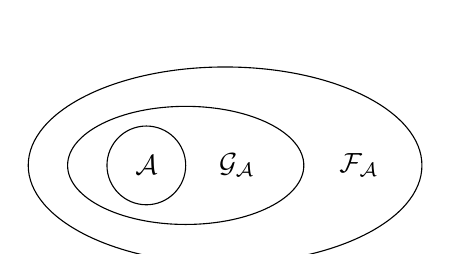
\begin{tikzpicture}
      \node at (0, 0) {$\mathcal{A}$};
      \node at (1.15, 0) {$\mathcal{G}_{\mathcal{A}}$};
      \node at (2.7, 0) {$\mathcal{F}_{\mathcal{A}}$};
      \draw (0, 0) circle [radius=0.5];
      \draw (0.5, 0) ellipse (1.5 and 0.75);
      \draw (1, 0) ellipse (2.5 and 1.25);
    \end{tikzpicture}
  \end{equation*}

  Now the hard part: to show that $\mathcal{F}_{\mathcal{A}} \subset \mathcal{G}_{\mathcal{A}}$. To do this we need to show that $\mathcal{G}_{\mathcal{A}}$ is a $\sigma$-algebra, i.e.\ contains $\Omega$ and is closed under countable unions and complements. If this is true then it is a $\sigma$-algebra containing $\mathscr{A}$, hence certainly contains the smallest $\sigma$-algebra containing $\mathscr{A}$.

  Our work is made much easier by the following observation: we will be done if we can show that $\mathcal{G}_{\mathcal{A}}$ is an algebra (it is \emph{not} necessary to show that $\mathcal{G}_{\mathcal{A}}$ is a $\sigma$-algebra!). That is, if we can show closure under finite unions and intersections, countable unions and intersections will take care of themselves.

  Why is this? Note that to show that $\mathcal{G}_{\mathcal{A}}$ is closed under, for example, countable unions, we would have to show that for any ${\left\{ A_{i} \right\}}_{i \in \N} \subset \mathcal{G}_{\mathcal{A}}$,
  \begin{equation*}
    \bigcup_{i \in \N} A_{i} \in \mathcal{G}_{\mathcal{A}}.
  \end{equation*}
  We have the equality
  \begin{equation*}
    \bigcup_{i \in \N} A_{i} = \bigcup_{i \in \N}\left( \bigcup_{j=1}^{i} A_{j} \right).
  \end{equation*}
  The outside union is increasing and monotone, and hence in $\mathcal{G}_{\mathcal{A}}$ because $\mathcal{G}_{\mathcal{A}}$ is a monotone class; we only need to show that each of the inside unions are in $\mathcal{G}_{\mathcal{A}}$. But these are only finite unions!

  So we need only show that $\mathcal{G}_{\mathcal{A}}$ is an algebra, i.e.\ closed under binary unions, binary intersections, and complements. In each case, our strategy will be the same: for each property we want $\mathcal{G}_{\mathcal{A}}$ to have, we will show that the set of all sets which have this property contains $\mathcal{A}$ and is a monotone class, hence contains $\mathcal{G}_{\mathcal{A}}$. This will imply that all of the sets of $\mathcal{G}_{\mathcal{A}}$ have this property.
  \begin{itemize}
    \item \textbf{Complements:} Consider the set of all subsets of $\Omega$ whose complemements are in $\mathcal{G}_{\mathcal{A}}$. Let's call it $\mathcal{C}$.
      \begin{equation*}
        \mathcal{C} = \left\{ C \subset \Omega\,\big|\, C^{c} \in \mathcal{G}_{\mathcal{A}} \right\}
      \end{equation*}
      Certainly, $\mathcal{A}$ is in $\mathcal{C}$ since $\mathcal{A}$ is an algebra and $\mathcal{A} \subset \mathcal{G}_{\mathcal{A}}$.

      We can say more about $\mathcal{C}$: it is a monotone class! To see this, we need to show that for a sequence ${\left\{ A_{i} \right\}}_{i \in \N} \subset \mathcal{C}$,
      \begin{itemize}
        \item if $A_{1} \subset A_{2} \subset \cdots$, then
          \begin{equation*}
            \bigcup_{i \in \N} A_{i} \in \mathcal{C}.
          \end{equation*}

          In this case, we have $A_{1}^{c} \supseteq A_{2}^{c} \supseteq \cdots$, and
          \begin{equation*}
            \bigcup_{i \in \N} A_{i} = {\left( \bigcap_{i \in \N} A_{i}^{c} \right)}^{c}.
          \end{equation*}
          All the $A_{i}^{c}$ are in $\mathcal{G}_{\mathcal{A}}$ by definition of $\mathcal{C}$, and their countable monotone intersection is in $\mathcal{G}_{\mathcal{A}}$ since $\mathcal{G}_{\mathcal{A}}$ is a monotone class. Since $\mathcal{C}$ is the set of all sets whose complements are in $\mathcal{G}_{\mathcal{A}}$ and $\bigcap_{i \in \N} A_{i}^{c}$ is in $\mathcal{G}_{A}$, its complement $\bigcup_{i \in \N} A_{i}$ is in $\mathcal{G}_{\mathcal{A}}$.

        \item If $A_{1} \supseteq A_{2} \supseteq \cdots$, then
          \begin{equation*}
            \bigcap_{i \in \N} A_{i} \in \mathcal{C}.
          \end{equation*}
          The proof is identical, but with inclusions reversed.
      \end{itemize}

      We give only sketches of the proofs of the other two conditions, as they are similar to the first case.

    \item \textbf{Finite unions:} By induction, we only need to prove closure under binary unions. So fix an arbitrary set $A \in \mathcal{A}$ and let $\mathcal{U}$ be the set of all subsets of $\Omega$ such that the union of $A$ and $B$ lands in $\mathcal{G}_{\mathcal{A}}$:
      \begin{equation*}
        \mathcal{U} = \left\{ B \subset \Omega\,\big|\, A \cup B \in \mathcal{G}_{\mathcal{A}} \right\}.
      \end{equation*}
      We omit the proof that this is indeed a monotone class.

    \item \textbf{Intersections:} As before, it suffices to show that
      \begin{equation*}
        \mathcal{I} = \left\{ B \subset \Omega\,\big|\, A \cap B \in \mathcal{G}_{\mathcal{A}} \right\}.
      \end{equation*}
      is a monotone class. We omit the proof of this.
  \end{itemize}
\end{proof}

\section{Some definitions from topology}
In the previous definitions, we have seen parallels between measure theory and topology. In what follows, one of our main goals will be to investigate the ways in which measure theory and topology interact. To do this, we will need definitions and results from topology in earnest. However, this is not a topology course, and we will not have time to go into topology, nor can we assume a working knowledge of it. In this section we give some working definitions, so we can get on with measure theory.

\begin{definition}[open set]
  \label{def:openset}
  A subset $O$ of the real line is \defn{open} if it is a union of open intervals.
\end{definition}

\begin{definition}[closed set]
  \label{def:closedset}
  A subset $C$ of the real line is \defn{closed} if its complement is open.
\end{definition}

\begin{theorem}
  If a subset $O \subset \R$ is open, then it can be expressed as a countable union of disjoint open intervals.
\end{theorem}

\begin{definition}[Borel $\sigma$-algebra]
  \label{def:borelsigmaalgebra}
  Let $(X, \tau)$ be a topological space. The $\sigma$-algebra generated by the open sets $\tau$ is called the \defn{Borel $\sigma$-algebra}.
\end{definition}

\section{Measures and measure spaces}
\subsection{Abstract measures}
\begin{definition}[abstract measure]
  \label{def:abstractmeasure}
  Let $(\Omega, \mathcal{F})$ be a measurable space. A \defn{measure} on $(\Omega, \mathcal{F})$ is a function $\mu\colon \mathcal{F} \to \R^{\geq 0}$ such that for any pairwise disjoint sequence $A_{i} \in \mathcal{F}$, we have
  \begin{equation*}
    \mu\left( \bigcup_{i \in \N} A_{i} \right) = \sum_{i \in \N} \mu(A_{i}).
  \end{equation*}

  The above condition is known as \emph{countable additivity}.
\end{definition}

\begin{note}
  In general, one also has the condition $\mu(\emptyset) = 0$ to ensure that $\mu( \emptyset ) \neq \infty$, but we do not demand this in this class for some reason.
\end{note}

\begin{example}
  \label{eg:diracmeasure}
  Consider a general measure space $(\Omega, \mathcal{F})$, and let $a \in \Omega$. Then the function
  \begin{equation*}
    \delta_{a}\colon \mathcal{F} \to \R^{+};\qquad A \mapsto
    \begin{cases}
      1, &a \in A \\
      0, &a \notin A
    \end{cases}
  \end{equation*}
  is a measure, called the \emph{Dirac measure}.
\end{example}

\begin{definition}[measure space]
  \label{def:measurespace}
  A \defn{measure space} is a triple $(\Omega, \mathcal{F}, \mu)$, where $(\Omega, \mathcal{F})$ is a measurable space (\hyperref[def:measurablespace]{Definition~\ref*{def:measurablespace}}) and $\mu$ is a measure on $(\Omega, \mathcal{F})$.
\end{definition}

\begin{example}
  \label{eg:discretemeasurespace}
  With $\Omega = \N$, $\mathcal{F} = 2^{\Omega}$, and $\mu(A) = \abs{A}$, $(\Omega, \mathcal{F}, \mu)$ is a measure space.
\end{example}

\subsection{Lebesgue measure}
The Lebesgue measure is a special case of the more general notion of measure defined above, which takes place on the real numbers $\R$.
\begin{definition}[outer measure]
  \label{def:outermeasure}
  For any subset $S \subset \R$, define the \defn{outer measure} $\mu^{*}$ of $S$ to be
  \begin{equation*}
    \mu^{*}(S) = \inf\left( \sum_{i \in I}\ell(I_{i}) \right),
  \end{equation*}
  where the infimum is taken over all coverings of $S$ by countably many intervals $I_{i}$.
\end{definition}

The idea is this: we imagine trying to cover our set $S$ by sets whose measure we `know': intervals. It may be helpful to picture papier-m\^{a}ch\'{e}. Since each covering of our set by intervals contains our set, the measure of our set should certainly not be greater than the measure of the cover. Thus, the total length of all the intervals comprising such a cover should give us an upper bound for the measure of the set. We define the `outer measure' to be the total length of the smalles covering, or more precisely the supremum of the lengths of all such coverings.

\begin{definition}[null set]
  \label{def:nullset}
  A \defn{null set} is a set $N$ for which
  \begin{equation*}
    \mu^{*}(N) = 0.
  \end{equation*}

  Here is a more explicit way of phrasing this defintion: A set $N$ is null if for any $\varepsilon > 0$ there exists a countable covering of $N$ by intervals of total length $\leq \varepsilon$.
\end{definition}

\begin{definition}[measurable set]
  \label{def:measurableset}
  A set $E \subset \R$ is \defn{measurable} if for any set $A \in \R$,
  \begin{equation*}
    \mu^{*}(A) = \mu^{*}(A \cap E) + \mu^{*} (A \cap E^{c}).
  \end{equation*}

  The set of all measurable sets is denoted $\mathcal{M}$.

  This condition is also known as the \emph{Carath\'{e}odory criterion}.
\end{definition}

\begin{note}
  Roughly speaking, the reasoning behind the definition of a measurable set is as follows. A set $E$ is measurable if it is regular enough that it can act as a screen in the following way: for \emph{any} set $A$, the outer measure of $A$ is equal to the outer measure of the part of $A$ which is hidden by the screen plus the outer measure part of $A$ which is visible.

  There is also a more `high-brow' way of viewing the above definition, which can be seen in, for example,~\cite{measurablesetsarelimitpoints}. In this approach, measurable sets in the above sense are shown to be the limit points of the collection of so-called `elementary sets,' i.e.\ sets which are expressible as a finite union of intervals.

  Practically speaking, encountering a non-measurable set `in the wild' is extraordinarily rare, and their construction generally involves the invocation of such arcanities as the axiom of choice. The following is an example of a non-measurable set.
\end{note}

\begin{example}
  Consider the group action on the circle $S^{1}$ by the group $G$ of rational rotations, i.e.\ rotations by an angle
  \begin{equation*}
    2\pi \cdot q,\qquad q \in \Q \cap \interval[open right]{0}{2\pi}.
  \end{equation*}

  The group $G$ is countable; in fact it is isomorphic to $\Q/\Z$. Thus, the orbit of any point on the circle is countable, and the group action partitions $S^{1}$ into uncountably many disjoint orbits $X_{i}$. From this partition, we can create our non-measurable set as follows.

  Using the axiom of choice, pick one representative $x_{i}$ from each orbit $X_{i}$. This gives us an uncountable subset $Z = \bigcup_{i} \{ x_{i} \} \subset S^{1}$. Acting on $Z$ with each element of $G$ in turn gives us all of $S^{1}$, so the images of $Z$ under rational rotation form a countable partition of $S^{1}$. Since these images are obtained from each other by rotation, any rotationally invariant measure on $S^{1}$ would assign them the same measure.

  Assigning any positive measure to $Z$ would not do since countable additivity would imply that the measure of $S^{1}$ was infinite, but they also cannot be of measure zero because then by countable additivity, $S^{1}$ would have measure zero. Hence, $Z$ cannot be measurable for any rotationally invariant measure on $S^{1}$.
\end{example}

\begin{definition}[Lebesgue measure]
  \label{def:lebesguemeasure}
  For any Lebesgue measurable set $M \in \mathcal{M}$, we write
  \begin{equation*}
    m(M) = \mu^{*}(M),
  \end{equation*}
  and call $m(M)$ the \defn{Lebesgue measure} of $M$.
\end{definition}

\begin{theorem}
  \label{thm:nullsetsandintervalsarelebesguemeasurable}
  $\,$
  \begin{enumerate}
    \item Any null set $N$ is neasurable and $m(N) = 0$.

    \item Any interval $\left\langle a, b \right\rangle$ is measureable and the measure is $b-a$.
  \end{enumerate}
\end{theorem}
\begin{proof}
  $\,$
  \begin{enumerate}
    \item If $N$ is a null set, then there is a cover $I_{n}$ of $N$ by intervals such that
      \begin{equation*}
        \sum_{n \in \N} \ell(I_{n}) = 0.
      \end{equation*}

      For any set $A \subset \R$, the intervals also cover $N \cap A$ and $N \cap A^{c}$, so both of these are null sets. But then
      \begin{equation*}
        m^{*}(N \cap A) + m^{*}(N \cap A^{c}) = 0 = m(N),
      \end{equation*}
      so $N$ is measurable.

    \item The interval $I = [a, b]$ covers itself, so outer measure of $I$ is at most $b - a$. To see that it cannot be any less, let $A_{i}$ be a covering of $I$ by intervals whose total length is less than $b-a$. Expanding the $i$th interval $A_{i}$ by $\frac{\varepsilon}{2^{i}}$, we can replace it with an open interval while still covering $I$. This gives us an open cover of a compact set, which has a finite sub cover $\tilde{A}_{i}$ $i = 1$, $2, \ldots n$.
  \end{enumerate}
\end{proof}

\begin{theorem}
  The Lebesgue measurable subsets $\mathcal{M}$ form a $\sigma$-algebra.
\end{theorem}
\begin{proof}
  $\,$
  \begin{enumerate}
    \item For any set $A \subset \R$, $A \cap \R = A$ and $A \cap \R^{c} = \emptyset$, so
      \begin{equation*}
        m(A \cap \R) = m(A).
      \end{equation*}

    \item Suppose $E \in \mathcal{M}$. Then
      \begin{equation*}
        m(E) = m(E \cap A) + m(E \cap A^{c})
      \end{equation*}
      for any subset $A \subset \R$.
  \end{enumerate}
\end{proof}

\begin{corollary}
  \label{cor:fullsetsaremeasurable}
  Any full set is measurable.
\end{corollary}

Consider the definition of a measurable set: $E$ is measurable if, for every set $A$,
\begin{equation*}
  m^{*}(A) = m^{*}(A \cap E) + m^{*}(A \cap E^{c}).
\end{equation*}
It is easy to show that any element of the Borel $\sigma$-algebra is measurable. There are elements of the Borel $\sigma$-algebra which have measure zero. But \emph{any} subset of such a set will be a null set, and hence Lebesgue measurable. This is an indication of the fact that there are more Lebesgue measurable sets than there are sets in the Borel $\sigma$-algebra.

\begin{definition}[completion of $\sigma$-algebra]
  \label{def:completionofsigmaalgebra}
  The \defn{completion} of a $\sigma$-algebra $\mathcal{G}$ w.r.t.\ a measure $\mu$ is the smallest $\sigma$-algebra containing $\mathcal{G}$ such that if $G \in \mathcal{G}$ and $\mu(G) = 0$ then $N \in \mathcal{G}$ for all $N \subset G$.
\end{definition}

\begin{theorem}
  The $\sigma$-algebra of Lebesgue-measurable subsets of $\R$ is the completion of the Borel $\sigma$-algebra w.r.t.\ the Lebesgue measure.
\end{theorem}

\section{Probability spaces}\label{sec:probabilityspaces}
Measure theory was originally developed to deal with the problem of finding a consistent way to assign `volumes' to subsets of a set. It was soon realized by Kolmogorov that the notion of a measure provided the correct way to assign probabilities to different outcomes in a consistent way. Thus the notion of a probability space was born.

\begin{definition}[probability space]
  \label{def:probabilityspace}
  A \defn{probability space} is a measure space $(\Omega, \mathcal{F}, P)$ such that $P(\Omega) = 1$.
\end{definition}

\begin{example}
  The measure space $\left( [0, 1], \mathcal{M}_{[0, 1]}, m \right)$ is a probability space since $m([0, 1]) = 1$.
\end{example}

\begin{example}
  Consider the measure space $(\R, \mathcal{M}, m)$, where $\mathcal{M}$ is the $\sigma$-algebra of Lebesgue measurable subsets of $\R$ and $m$ is the Lebesgue measure. Pick some $B \in \mathcal{M}$.

  Let
  \begin{equation*}
    \mathcal{M}_{B} = \left\{ A \cap B\,\big|\, A \in \mathcal{M} \right\}.
  \end{equation*}
  Then $\mathcal{M}_{B}$ is a $\sigma$-algebra on $B$. If, for $X \in \mathcal{M}_{B}$ we define $P(X) = \frac{m(X)}{m(B)}$, then $P$ is a probability measure, so $(B, \mathcal{M}_{B}, P)$ is a probability space.
\end{example}

\begin{example}
  Let $(\Omega, \mathcal{F}, P)$ be a probability space. Let $B \in \mathcal{F}$. Then for any set $A \in \mathcal{F}$ we define the \emph{conditional probability} $P(A | B)$ as follows:
  \begin{equation*}
    P(A | B) = \frac{P(A \cap B)}{P(B)}.
  \end{equation*}

  In fact, $P(\,\cdot\,|B)$ is also a probability measure on $(\Omega, \mathcal{F})$.
\end{example}

\section{Independent \texorpdfstring{$\sigma$}{Lg}-algebras}

\begin{definition}[independent $\sigma$-algebras]
  \label{def:independentsigmaalgebra}
  Let $(\Omega, \mathcal{F}, P)$ be a probability space. Two $\sigma$-algebras $\mathcal{F}_{1}$, $\mathcal{F}_{2} \subset \mathcal{F}$ are \defn{independent} if for any $A_{1} \in \mathcal{F}_{1}$ and $A_{2} \in \mathcal{F}_{2}$,
  \begin{equation*}
    P(A_{1} \cap A_{2}) = P(A_{1}) \cdot P(A_{2}).
  \end{equation*}
\end{definition}

\begin{definition}[independent events]
  \label{def:independentevents}
  Let $(\Omega, \mathcal{F}, P)$ be a probability space. The events $A_{1}$, $A_{2}$, \dots, $A_{n} \in \mathcal{F}$ are \defn{independent} if for all $K \subset \left\{ 1,\ldots, n \right\}$,
  \begin{equation*}
    P\left( \bigcap_{k \in K} A_{k} \right) = \prod_{k \in K} P(A_{k}).
  \end{equation*}
\end{definition}

\begin{example}
  Suppose $A$ and $B$ are independent events. Then the $\sigma$-algebras they generate,
  \begin{equation*}
    \mathcal{F}_{A} = \left\{ \emptyset, A, A^{\mathrm{c}}, \Omega \right\}\qquad\text{and}\qquad\mathcal{F}_{B}=\left\{ \emptyset, B, B^{\mathrm{c}}, \Omega \right\}
  \end{equation*}
  are independent since
  \begin{align*}
    P(A \cap B) &= P(A)\cdot P(B) &\left( \text{by definition} \right) \\
    P(A \cap B^{\mathrm{c}}) &= P(A) \cdot (1-P(B)) &\left( m(A \cap B) + m(A \cap B^{c}) = m(A) \right) \\
    P(A^{\mathrm{c}} \cap B) &= (1 - P(A))\cdot P(B) &\left( \text{by symmetry} \right) \\
    P(A^{\mathrm{c}} \cap B^{\mathrm{c}}) &= (1 - P(A)) \cdot (1-P(B)) &\left( m(A \cap B^{\mathrm{c}}) + m(A^{\mathrm{c}} \cap B^{c}) = m(A^{\mathrm{c}}) \right) \\
  \end{align*}
  and
  \begin{equation*}
    P(A^{\mathrm{c}}) = 1-P(A)\qquad\text{and}\qquad P(B^{c}) = 1-P(B).
  \end{equation*}
\end{example}

Independence of events is a bit nasty in the following way. Suppose we have three events $A$, $B$, and $C$. If $A$ and $B$ are independent, $A$ and $C$ are independent, and $B$ and $C$ are independent, it does not follow that $A$, $B$, and $C$ are independent. In other words, pairwise independence does not imply independence.

This is why we have to check all possible subsets $K$ of $\left\{ 1, \ldots, n \right\}$: we want events to be independent only if they are pairwise independent, triple-wise independent, etc.


\section{Measurable functions}
Certain unifying concepts lurk in the shadows behind almost every major event in modern mathematics. Possibly the most prevalent of these is the idea of a structure-preserving map. The idea is this: we have two objects $A$ and $B$ which have some structure (say, a topology, a binary operation, etc.), and we want to talk about maps $f\colon A \to B$ which preserve this structure. In the case where our structures are measurable spaces (\hyperref[def:measurablespace]{Definition~\ref*{def:measurablespace}}), we call the structure-preserving maps \emph{measurable}.

\begin{definition}[measurable map]
  \label{def:measurablefunction}
  Let $(\Omega, \mathcal{F})$ and $(\Omega', \mathcal{F}')$ be measurable spaces. A map $\Omega \to \Omega'$ is \defn{measurable} if for any $M \in \mathcal{F}'$, the set $f^{-1}(M) \in \mathcal{F}$.

  That is, $f$ is measurable if the preimage of every measurable set is measurable.
\end{definition}

\begin{lemma}
  \label{lemma:functionalsomeasurablewithrespecttobiggersigmaalgebra}
  Let $(\Omega, \mathcal{F})$ be a measure space, let $f$ be a measurable function on $(\Omega, \mathcal{F})$, and let $\mathcal{F} \subset \mathcal{G}$. Then $f$ is $\mathcal{G}$-measurable.
\end{lemma}
\begin{proof}
  Let $\mathcal{B}$ be a measurable set in the codomain of $f$. Then since $f$ is $\mathcal{F}$-measurable, $f^{-1}(B) \in \mathcal{F}$. But since $\mathcal{F} \subset \mathcal{G}$, $f^{-1}(B) \in \mathcal{G}$, so $f$ is also $\mathcal{G}$-measurable.
\end{proof}

For the purposes of this course, we will mainly be interested in maps between (Lebesgue measurable) subsets of $\R$. In this case we have the following definition.
\begin{definition}[Lebesgue measurable function]
  \label{def:lebesguemeasurablefunction}
  Let $E \in \mathcal{M}$. A function $f\colon E \to \R$ is \defn{Lebesgue measurable} if the preimage of every Lebesgue measurable subset is Lebesgue is measurable.
\end{definition}

\begin{theorem}
  The following are equivalent:
  \begin{enumerate}
    \item The map $f$ is Lebesgue measurable

    \item The preimage under $f$ of every Borel set is Lebesgue measurable

    \item The preimage under $f$ of every open set is Lebesgue measurable

    \item The preimage under $f$ of every closed set is Lebesgue measurable

    \item the preimave under $f$ of every interval is Lebesgue measurable.

    \item The preimage under $f$ of each set of the form $(-\infty, A)$ is Lebesgue measurable.
  \end{enumerate}
\end{theorem}

The set of functions $E \to \R$ forms an $\R$-algebra with addition and multiplication defined pointwise. It turns out that the Lebesgue measurable functions form a subalgebra.
\begin{theorem}
  If $(\Omega, m)$ is a measure space, $f$ and $g$ are measurable functions $\Omega \to \R$, and $\lambda \in \R$, then the following functions are also measurable.
  \begin{itemize}
    \item $f + g$

    \item $fg$

    \item $\lambda f$
  \end{itemize}
\end{theorem}
\begin{proof}
  $\,$
  \begin{enumerate}
    \item We need to show that ${(f+g)}^{-1}[(-\infty, A)]$ is Lebesgue measurable for every $A \in \R$, i.e.\ that the set
      \begin{equation*}
        \left\{ x \in \R\,\big|\, f(x) + g(x) < A \right\}
      \end{equation*}
      is Lebesgue measurable.

      $f(x) + g(x) < A$ if and only there exists a rational number between $f(x) + g(x)$ and $A$, or equivalently between $g(x)$ and $A - f(x)$; call it $r$. Then $g(x) < r$ and $r < A - f(x)$, i.e.\ $f(x) > A - r$. Moreover, these inequalities are satisfied if and only if $r$ is between $g(x)$ and $A - f(x)$. Thus,
      \begin{equation*}
        \left\{ x\colon f(x) + g(x) < A \right\} = \bigcup_{q \in \R} \left( f^{-1}[(-\infty, r)] \cap g^{-1}[(-\infty, A-r)] \right).
      \end{equation*}

      The RHS is measurable because it is built from countable unions and intersections of sets which are measurable because $f$ and $g$ are.

    \item If we can show that for any measurable function $f$ the function $f^{2}$ is measurable, then we will be done since
      \begin{equation*}
        f\cdot g = \frac{1}{2}\left( {(f+g)}^{2} - {(f-g)}^{2} \right)
      \end{equation*}

      We need to show that the set
      \begin{equation*}
        \left\{ x \in \R\,\big|\, {f(x)}^{2} < A \right\}
      \end{equation*}
      is measurable for any $A$. But if $A \geq 0$ this is the same as the set
      \begin{equation*}
        \left\{ x \in \R \,\big|\, f(x) < \sqrt{A} \text{ or } f(x) > -\sqrt{A} \right\},
      \end{equation*}
      and if $A < 0$, this is the empty set, which is trivially measurable.

      Okay, so suppose $A \geq 0$. Then
      \begin{equation*}
        {(f^{2})}^{-1}[(-\infty, A)] = f^{-1}(-\sqrt{A}, \sqrt{A}),
      \end{equation*}
      which is the preimage of an interval and hence measurable.

    \item ${(\lambda f)}^{-1}([a, b]) = f^{-1}\left( \left[ \frac{a}{\lambda}, \frac{b}{\lambda} \right] \right)$.
  \end{enumerate}
\end{proof}

\begin{definition}[limit supremum, limit infimum]
  \label{def:limsupliminf}
  Let ${\left\{ z_{n} \right\}}_{n=1}^{\infty}$ be a sequence of real numbers. Then
  \begin{enumerate}
    \item $\displaystyle\limsup_{n \to \infty} z_{n} = \lim_{N \to \infty}\left( \sup_{n \geq N} z_{n} \right) = \inf_{N \geq 1}\left( \sup_{n \geq N} z_{n} \right)$;

    \item $\displaystyle\liminf_{n \to \infty} z_{n} = \lim_{N \to \infty}\left( \inf_{n \geq N} z_{n} \right) = \sup_{N \geq 1} \left(  \inf_{n \leq N} z_{n} \right)$;
  \end{enumerate}
\end{definition}
\begin{note}
  Here are more user-friendly `definitions' of the limit supremum and limit infimum of a sequence $z_{i}$: $\limsup_{n \to \infty} z_{n}$ is the largest number that any subsequence of $z_{n}$ can converge to; $\liminf_{n \to \infty}$ is the smallest.
\end{note}

\begin{lemma}
  \label{lemma:limsupofnegativeisnegativeliminf}
  Let $a_{n}$ be a sequence of numbers. Then
  \begin{itemize}
    \item $\limsup_{n \to \infty} (- a_{n}) = - \liminf_{n \to \infty} a_{n}$, and
    \item $\liminf_{n \to \infty} (- a_{n}) = - \limsup_{n \to \infty} a_{n}$.
  \end{itemize}
\end{lemma}
\begin{proof}
  We prove the first equality. The proof of the second is identical.
  \begin{align*}
    \limsup_{n \to \infty} (-a_{n}) &= \lim_{N \to \infty}\left( \sup_{n \geq N} (-a_{n}) \right) \\
    &= \lim_{N \to \infty} \left( -\inf_{n \geq N} a_{n} \right) \\
    &= -\lim_{N \to \infty} \left( \inf_{n \geq N} a_{n} \right) \\
    &= -\liminf_{n \to \infty} a_{n}.
  \end{align*}
\end{proof}

\begin{theorem}
  \label{thm:limitsoffunctionsaremeasurable}
  Let $\left\{ f_{n} \right\}$ be a sequence of measurable functions. Then
  \begin{enumerate}
    \item $f_{M}(x) = \max_{n \leq k} f_{n}(x)$

    \item $f_{m}(x) = \min_{n \leq k} f_{n}(x)$

    \item $f_{s}(x) = \sup_{n \in \N} f_{n}(x)$

    \item $f_{i}(x) = \inf_{n \in \N} f_{n}(x)$

    \item $f_{ls}(x) = \liminf_{n \in \N} f_{n}(x)$

    \item $f_{li}(x) = \limsup_{n \in \N} f_{n}(x)$
  \end{enumerate}
  are all measurable.
\end{theorem}

\begin{corollary}
  If a sequence of measurable functions converges pointwise then the function to which the sequence converges is measurable.
\end{corollary}

\begin{theorem}
  Let $(\Omega, \mathcal{M})$ be a measurable space. Let $E \in \mathcal{M}$, $f\colon E \to \R$ be measurable, and $g\colon E \to \R$ be a function which is equal to $f$ almost everywhere. Then $g$ is measurable.
\end{theorem}
\begin{proof}
  The difference $g - f$ is equal to zero almost everywhere. Consider the preimage
  \begin{equation*}
  \mathrm{preim}_{g-f}\left( \interval[open left]{-\infty}{a} \right),
\end{equation*}

Since $g - f$ is zero almost everywhere, this is a null set if $a < 0$, and a full set if $a \geq 0$. Both null sets and full sets are measurable, so $g - f$ is measurable. But then $(g - f) + f = g$ is measurable.
\end{proof}

\begin{corollary}
  Suppose that a sequence of measurable functions $f_{n}$ converge to a function $f$ almost everywhere. Then $f$ is measurable.
\end{corollary}
\begin{proof}
  Denote the set on which $f_{n}$ converges to $f$ by $S$. Then $f_{n}\cdot\mathbb{I}_{S}$ converges everywhere to $f\cdot\mathbb{I}_{S}$. But $f$ and $f\cdot \mathbb{I}_{S}$ agree almost everywhere, so $f$ agrees with a measurable function almost everywhere, hence is itself measurable.
\end{proof}

\section{Random variables}
Measurable functions on probability spaces have a special name.

\begin{definition}[random variable]
  \label{def:randomvariable}
  Let $(\Omega, \mathcal{F}, P)$ be a probability space. A \defn{random variable} $X$ is a measurable function $\Omega \to \R$.
\end{definition}

As we saw in \hyperref[sec:probabilityspaces]{Section~\ref*{sec:probabilityspaces}}, probability spaces $(\Omega, \mathcal{F}, P)$ encode the idea of a space of events and the probabilities that they occur. A random variable should be thought of as associating a number to each event.

\begin{example}
  Consider the probability space $(\Omega, \mathcal{M}, P)$ where
  \begin{equation*}
    \Omega = \{ 1, 2, 3, 4, 5, 6 \};\qquad \mathcal{M} = 2^{\Omega};\qquad P(A) = \frac{\abs{A}}{6}.
  \end{equation*}

  This is the probability space that encodes the notion of a fair die roll.

  An example of a random variable is
  \begin{equation*}
    X\colon \Omega \to \R;\qquad X(\omega) =
    \begin{cases}
      0, &\omega\text{ even} \\
      1, &\omega\text{ odd}.
    \end{cases}
  \end{equation*}

  A possibly simpler example is
  \begin{equation*}
    Y(\omega) = \omega,
  \end{equation*}
  which assigns to each possible outcome the value on the die.
\end{example}

\begin{theorem}
  \label{thm:preimageofsigmaalgebraissigmaalgebra}
  Let $(\Omega, \mathcal{F}, P)$ be a probability space, $X$ a random variable. The family of sets
  \begin{equation*}
    \left\{ S \in \mathcal{F}\,\big|\, S = X^{-1}(B)\text{ for some }B \in \mathcal{B} \right\} \equiv X^{-1}(\mathcal{B}),
  \end{equation*}
  where $\mathcal{B}$ is the Borel $\sigma$-algebra on $\R$, is a $\sigma$-algebra.
\end{theorem}
\begin{proof}
  We need to show that (1) $\Omega \in X^{-1}(\mathcal{B})$, (2) $X^{-1}(\mathcal{B})$ is closed under complements, and (3) $X^{-1}(\mathcal{B})$ is closed under countable unions.
  \begin{enumerate}
    \item $\Omega \in \mathcal{F}$ and $\Omega = X^{-1}(\R)$.

    \item Let $A \in X^{-1}(\mathcal{B})$. Then $A = X^{-1}(B)$ for some $B \in \mathcal{B}$, so $A^{c} = X^{-1}(B^{c})$.

    \item Let $A_{i} \in X^{-1}(\mathcal{B})$, $i \in \N$. Then for each $i$, $A_{i} = X^{-1}(B_{i})$ for some Borel set $B_{i} \in \mathcal{B}$.

      Claim:
      \begin{equation*}
        \bigcup_{i \in \N} A_{i} = X^{-1}\left( \bigcup_{i \in \N} B_{i} \right).
      \end{equation*}

      If $x \in \bigcup_{i \in \N} A_{i}$, then $x$ is in the preimage of at least one of the $B_{i}$, say $B_{n}$. Therefore it is in the preimage of any set which contains that $B_{n}$, such as $X^{-1}\left( \bigcup_{i \in \N}B_{i} \right)$.

      Now, suppose that $x \in X^{-1}\left( \bigcup_{i \in \N} B_{i} \right)$. Then its image under $X$ is in $\bigcup_{i \in \N} B_{i}$, i.e.\ it is in at least one of the $A_{i}$, say $A_{m}$. Then it is in the union of all the $A_{m}$.

      Then we are done, since $\bigcup_{i \in \N} B_{i} \in \mathcal{B}$.
  \end{enumerate}
\end{proof}

\begin{definition}[sigma-algebra generated by a random variable]
  \label{def:sigmaalgebrageneratedbyarandomvariable}
  For $(\Omega, \mathcal{F}, P)$ a probability space and $X\colon \Omega \to \R$ a random variable, the \defn{$\sigma$-algebra generated by $X$} is the $\sigma$-algebra
  \begin{equation*}
    X^{-1}(\mathcal{B})
  \end{equation*}
  from \hyperref[thm:preimageofsigmaalgebraissigmaalgebra]{Theorem~\ref*{thm:preimageofsigmaalgebraissigmaalgebra}}.
\end{definition}

\begin{example}
  Let $(\Omega, \mathcal{F})$ be a measure space, $f\colon \Omega \to \R$ the constant function
  \begin{equation*}
    f(x) = a.
  \end{equation*}

  Then the $\sigma$-algebra generated by $f$ is the trivial $\sigma$-algebra $\{\emptyset, \Omega\}$.
\end{example}

\begin{example}
  \label{eg:sigmaalgebrageneratedbytwovaluedfunction}
  Let $\Omega = [0, 1]$. Consider the measurable space $(\Omega, \mathcal{B}_{[0, 1]})$.

  Let $X$ be a random variable defined by
  \begin{equation*}
    X(\omega) =
    \begin{cases}
      a, &\omega \in \interval[open right]{0}{\frac{1}{4}} \cup \interval[open right]{\frac{1}{2}}{\frac{3}{4}} \\
      b, &\omega \in \interval[open right]{\frac{1}{4}}{\frac{3}{4}} \cup \interval{\frac{3}{4}}{1}
    \end{cases},
  \end{equation*}
  with $a \neq b$.

  For any borel set $B \in \mathcal{B}$, $X^{-1}(B)$ can take one of four values.
  \begin{itemize}
    \item $X^{-1}(B) = \emptyset$ if $a \notin B$ and $b \notin B$.

    \item $X^{-1}(B) = \interval[open right]{0}{\frac{1}{4}} \cup \interval[open right]{\frac{1}{2}}{1}$, if $a \in B$ and $b \notin B$.

    \item $X^{-1}(B) = \interval[open right]{\frac{1}{4}}{\frac{1}{2}} \cup \interval{\frac{3}{4}}{1}$, if $a \notin B$ and $b \in B$

    \item $X^{-1}(B) = \Omega$ if $a \in B$ and $b \in B$.
  \end{itemize}

  Therefore, the $\sigma$-algebra $\mathcal{F}_{X}$ generated by $X$ is given by
  \begin{equation*}
    \mathcal{F}_{X} = \left\{ \emptyset, \interval[open right, scaled]{0}{\frac{1}{4}} \cup \interval[open right, scaled]{\frac{1}{2}}{\frac{3}{4}}, \interval[open right, scaled]{\frac{1}{4}}{\frac{1}{2}} \cup \left[\frac{3}{4}, 1\right], \Omega \right\}.
  \end{equation*}
\end{example}

Here is an interpretation of the above results: \emph{The size of the $\sigma$-algebra generated by a random variable tells you how much information the measurement of that random variable gives you.}
\begin{example}
  $\,$
  \begin{itemize}
    \item If $X$ is the constant random variable $X(\omega) = a$, then $X^{-1}(\mathcal{B}) = \{\emptyset, \Omega\}$. This is the smallest $\sigma$-algebra there is. Morally speaking this happens, because measuring the value of a constant function tells you nothing.

    \item The $\sigma$-algebra generated by the identity function on $(\R, \mathcal{B})$ is equal to $\mathcal{B}$. This is the biggest $\sigma$-algebra one could get. Morally, this happens because if you know the value of the identity function where you're standing, you know where you are. The same is true of any injection.

    \item The $\sigma$-algebra generated by the random variable
      \begin{equation*}
        X\colon [0, 1] \to \R;\qquad \omega \mapsto
        \begin{cases}
          0, &\omega \in \interval[open right]{0}{\frac{1}{2}} \\
          1, &\omega \in \interval{\frac{1}{2}}{1}
        \end{cases}
      \end{equation*}
      is
      \begin{equation*}
        \mathcal{F}_{X} = \left\{ \emptyset, \interval[open right]{0}{\frac{1}{2}}, \left[ \frac{1}{2}, 1 \right], \Omega \right\}
      \end{equation*}
      which reflects the fact that a measurement of $X$ can tell you which side of $[0, 1]$ you're on, but never more than that.

    \item The sets in the $\sigma$-algebra generated by an even function contain subsets of the form $\{x, -x\}$, but never $x$ without $-x$. This reflects the fact that if you measure the value of an even function, you don't know which side of the origin you're on.
  \end{itemize}
\end{example}

\begin{definition}[independent random variables]
  \label{def:independentrandomvariables}
  Let $(\Omega, \mathcal{F}, P)$ be a probability space. Random variables $X_{1}$, $X_{2}$, \ldots, $X_{n}$ are \emph{independent} if the $\sigma$-algebras generated by them are mutually independent, i.e.\ if for any $B_{1}$, $B_{2}$, \ldots, $B_{n} \in \mathcal{B}$,
  \begin{equation*}
    P\left( \bigcap_{i = 1}^{n} X^{-1}(B_{i}) \right) = \prod_{i = 1}^{n} P(X_{i}^{-1}(B_{i})).
  \end{equation*}
\end{definition}

Here is an interpretation of the above results: \emph{Two random variables are independent if measuring the value of one tells you nothing about measuring the value of the other.} To see this a bit more clearly, consider the case of two independent random variables $X$ and $Y$. We say that $X$ and $Y$ are independent if for each $A, B \in \mathcal{B}$,
\begin{equation*}
  P\left( X^{-1}(A) \cap Y^{-1}(B) \right) = P\left( X^{-1}(A) \right)\cdot P\left( Y^{-1}(B) \right).
\end{equation*}

Sets of the form $X^{-1}(A)$ are exactly those which belong to $\mathcal{F}_{X}$, so we could equally say: $X$ and $Y$ are independent if for any events $C \in \mathcal{F}_{X}$ and $D \in \mathcal{F}_{D}$,
\begin{equation*}
  P(C \cap D) = P(C)\cdot P(D).
\end{equation*}

We can re-arrange this to say that $X$ and $Y$ are independent if and only if
\begin{equation*}
  P(C | D) = P(C)\qquad\text{and}\qquad P(D |C) = P(D)\qquad\text{for any }C \in \mathcal{F}_{X}, D \in \mathcal{F}_{Y}.
\end{equation*}

Note that the definition is symmetric: we say that $X$ and $Y$ are independent, not $X$ is independent of $Y$.

\begin{example}
  \label{eg:independentstepfunctions}
  Consider the probability space $\left( [0, 1], \mathcal{M}_{[0, 1]}, m \right)$, and the random variables
  \begin{equation*}
    X(\omega) =
    \begin{cases}
      0, &\omega \in \interval[open right]{0}{\frac{1}{2}} \\
      1, &\omega \in \left[ \frac{1}{2}, 1 \right]
    \end{cases},
    \qquad
    Y(\omega) =
    \begin{cases}
      0, & \omega \in \interval[open right]{0}{\frac{1}{4}} \cup \interval[open right]{\frac{1}{2}}{\frac{3}{4}} \\
      1 & \omega \in \interval[open right]{\frac{1}{4}}{\frac{1}{2}} \cup \left[ \frac{3}{4}, 1 \right]
    \end{cases}.
  \end{equation*}

  It is easy to check that the $\sigma$-algebras generated by $X$ and $Y$ are independent. This is intuitively because of the following:

  A priori each value of $Y$ is equally likely since
  \begin{equation*}
    m\left( \interval[open right, scaled]{0}{\frac{1}{4}} \cup \interval[open right, scaled]{\frac{1}{2}}{\frac{3}{4}} \right) = m\left( \interval[open right, scaled]{\frac{1}{4}}{\frac{1}{2}} \cup \interval[open right, scaled]{\frac{3}{4}}{1} \right) = \frac{1}{2}.
  \end{equation*}
  If we measure, say, $X = 0$, then the probability of either outcome is still $\frac{1}{2}$, and similarly $X = 1$, $Y = 0$, and $Y = 1$.
\end{example}

\begin{example}
  Suppose we have two random variables $X$ and $Y$ such that
  \begin{equation*}
    \mathcal{F}_{X} = \mathcal{F}_{Y}.
  \end{equation*}

  These random variables are not \emph{necessarily} dependent, but their structure is constrained. For any $A \in \mathcal{F}_{X}$, we have
  \begin{equation*}
    P(A) = P(A \cap A) = P(A)\cdot P(A),
  \end{equation*}
  i.e.\ $P(A) = 0$ or $P(A) = 1$ for all $A \in \mathcal{F}_{X}$.
\end{example}

\section{Probability distributions}
\begin{definition}[probability distribution of a random variable]
  \label{def:probabilitydistributionofrandomvariable}
  Let $(\Omega, \mathcal{F}, P)$ be a probability space, $X\colon \Omega \to \R$ be a random variable. The \emph{probability distribution defined by $X$}, denoted $P_{X}$, is the measure on $(\R, \mathcal{B})$ defined by
  \begin{equation*}
    P_{X}(B) = P(X^{-1}(B)).
  \end{equation*}
  That is, $P_{X}\colon \mathcal{B} \to \R$.
\end{definition}

The value of a probability distribution $P_{X}(B)$ of a random variable $X$ tells you the probability that the outcome of a measurement of the value of $X$ lies somewhere in a set $B$.

\begin{theorem}
  Let $(\Omega, \mathcal{F}, P)$ be a probability space, $X\colon \Omega \to \R$ be a random variable. Then $P_{X}$ is a probability measure, i.e.\ $(\R, \mathcal{B}, P_{X})$ is a probability space.
\end{theorem}
\begin{proof}
  Non-negativity is obvious, and $P_{X}(\R) = P(X^{-1}(\R)) = P(\Omega) = 1$, so we need only show that if $\{B_{i}\}$ is a countable, pairwise disjoint collection of Borel sets, then
  \begin{equation*}
    P_{X}\left( \bigcup_{i} B_{i} \right) = \sum_{i} P_{X}(B_{i}).
  \end{equation*}

  By definition,
  \begin{equation*}
    P_{X}\left( \bigcup_{i} B_{i} \right) = P\left( X^{-1}\left( \bigcup_{i} B_{i} \right) \right).
  \end{equation*}

  Since the $B_{i}$ are pairwise disjoint, so are $X^{-1}(B_{i})$. The result follows since $P$ is countably additive.
\end{proof}

\begin{example}
  Recall the function $X(\omega)$ from \hyperref[eg:sigmaalgebrageneratedbytwovaluedfunction]{Example~\ref*{eg:sigmaalgebrageneratedbytwovaluedfunction}}:
  \begin{equation*}
    X(\omega) =
    \begin{cases}
      a, &\omega \in \interval[open right]{0}{\frac{1}{4}} \cup \interval[open right]{\frac{1}{2}}{\frac{3}{4}} \\
      b, &\omega \in \interval[open right]{\frac{1}{4}}{\frac{1}{2}} \cup [\frac{3}{4}, 1]
    \end{cases},\qquad
    a \neq b.
  \end{equation*}

  The probability distribution generated by $X$, denoted $P_{X}$, has the following form. For any Borel measurable set $B$, $P_{X}(B) =$
  \begin{itemize}
    \item $P(\emptyset) = 0$ if $a \notin B$ and $b \notin B$.

    \item $P(\interval[open right]{0}{\frac{1}{4}} \cup \interval[open right]{\frac{1}{2}}{\frac{3}{4}}) = \frac{1}{2}$, if $a \in B$ and $b \notin B$.

    \item $P( \interval[open right]{\frac{1}{4}}{\frac{1}{2}} \cup \interval[open right]{\frac{3}{4}}{1} = \frac{1}{2}$, if $a \notin B$ and $b \in B$

    \item $P(\Omega) = 1$ if $a \in B$ and $b \in B$.
  \end{itemize}

  Thus, we could equally write
  \begin{equation*}
    P_{X} = \frac{1}{2}\left( \delta_{a} + \delta_{b} \right),
  \end{equation*}
  where $\delta_{(\cdot)}$ is the Dirac measure from \hyperref[eg:diracmeasure]{Example~\ref*{eg:diracmeasure}}.
\end{example}

\begin{example}
  \label{eg:probabilitygeneratedbycomplicatedishfunction}
  Consider the probability space $\left( [0, 1], \mathcal{M}_{[0, 1]}, m \right)$ and the random variable
  \begin{equation*}
    X(\omega) =
    \begin{cases}
      5\omega, & \omega \in \left[ 0, \frac{1}{3} \right] \\
      4, & \omega \in \left( \frac{1}{3}, \frac{2}{3} \right) \\
      5(1-\omega) & \omega \in \left[ \frac{2}{3}, 1 \right]
    \end{cases}.
  \end{equation*}

  First, we calculate $P_{X}$. The preimage of any set $A$ which is contained entirely in $\left[ 0, \frac{5}{3} \right]$ will be mapped to two places: $A/5$ and $1 - A/5$. Each of these is shrunk by a factor of 5, and there are two of them, so $P_{X}(A) = \frac{2}{5}m(A)$.

  If $A$ contains $4$ and does not have a component in $\left[ 0, \frac{5}{3} \right]$, then $X^{-1}(A)$ will contain the interval $\left( \frac{1}{3}, \frac{2}{3} \right)$.

  Thus,
  \begin{equation*}
    P_{X}(B) = \frac{1}{3}\delta_{4}(B) + \frac{2}{5} m\left( B \cap \left[ 0, \frac{5}{3} \right] \right).
  \end{equation*}
\end{example}

This makes sense intuitively: on $[0, \frac{1}{3}]$, $X$ stretches out sets by a factor of $5$ so preimages will be shrunk by $\frac{1}{5}$.

\begin{definition}[cumulative distribution function]
  \label{def:cumulativedistributionfunction}
  For any random variable $X$ on a probability space $(\Omega, \mathcal{F}, P)$, the \defn{cumulative distribution function}, or CDF, of $X$, denoted $F_{X}(t)$, is the real function
  \begin{equation*}
  F_{X}(t) = P_{X}(\interval[open left]{-\infty}{t}).
\end{equation*}
\end{definition}
\section{Integration}
The preliminary results of Lebesgue integration theory take rather a different form to those from Riemann integration. The most obvious difference is that many results from Lebesgue integration theory are proved only for non-negative measurable functions, and then extended to all measurable functions via positive decomposition. (See, for example, \hyperref[def:integrablefunctionlebesgueintegral]{Definition~\ref*{def:integrablefunctionlebesgueintegral}} for the definition of positive decomposition.)

\subsection{Simple functions}

\begin{definition}[simple function]
  \label{def:simplefunction}
  Let $E \subset \R$. A non-negative function $\varphi\colon E \to \R$ is \defn{simple} if it is measurable and takes on only finitely many values $a_{1}$, $a_{2}$, \ldots, $a_{n}$. Equivalently, a function $\varphi$ which takes on finitely many values $a_{i}$ is simple if each preimage $\varphi^{-1}(\{a_{i}\})$ is measurable.
\end{definition}

\begin{definition}[lebesgue integral of a simple function]
  \label{def:lebesgueintegralofsimplefunction}
  Let $(\R, \mathcal{M}, m)$ be a measure space, let $E \subset \mathcal{M}$, and let $\varphi\colon E \to \R$ be a simple function. Let $ \varphi^{-1}\left( \{ a_{i} \} \right) = A_{i}$. The \defn{Lebesgue integral} of $\varphi$ over $E$ is defined by
  \begin{equation*}
    \int_{E} \varphi\ dm = \sum_{i} a_{i}\cdot m(A_{i} \cap E).
  \end{equation*}
\end{definition}

\begin{note}
  We explicitly allow the case in which $\int_{E} \varphi\ dm = \infty$. This is in stark contrast to the usual treatment, and will come back to bite us in the rear end when we define the Lebesgue integral for general measurable functions in \hyperref[def:integrablefunctionlebesgueintegral]{Definition~\ref*{def:integrablefunctionlebesgueintegral}}; see \hyperref[note:perniciouslittlecorner]{Note~\ref*{note:perniciouslittlecorner}} for more details.
\end{note}

\begin{example}
  Recall the function
  \begin{equation*}
    f\colon \R \to \R;\qquad f(x) =
    \begin{cases}
      1, &x \in \Q \\
      0, &x \notin \Q
    \end{cases}.
  \end{equation*}

  The function $f$ is measurable since the preimage of any (measurable) set is either null or full and hence measurable, and simple since it takes on only finitely many values (0 and 1). Its Lebesgue integral is
  \begin{equation*}
    \int_{\R} f\ dm = 0\cdot m(\R \setminus \Q) + 1 \cdot m(\Q) = 0.
  \end{equation*}

  This function is not Riemann integrable!
\end{example}

\subsection{Integration of non-negative measurable functions}
\begin{definition}[Legesgue integral of a non-negative measurable function]
  \label{def:lebesgueintegralofnonnegativemeasurablefunction}
  Let $E \in \mathcal{M}$, $f\colon E \to \R$ be a measurable function. The \defn{Lebesgue integral} of $f$ over $E$ is
  \begin{equation*}
    \sup_{\varphi \in \Phi(f, E)} \int_{E} \varphi\ dm,
  \end{equation*}
  where $\Phi(f, E) = \left\{ \varphi\colon E \to \R \text{ simple and }0 \leq \varphi(x) \leq f(x)\text{ for all }x \in E \right\}$.
\end{definition}

\begin{example}
  \label{eg:lebesgueintegralcanbesum}
  Consider the measure space $(\Omega = \N, \mathcal{F} = 2^{\N}, \mu = \abs{\cdot})$ from \hyperref[eg:discretemeasurespace]{Example~\ref*{eg:discretemeasurespace}}. Any non-negative function $f\colon \N \to \R$ is measurable, and the integral
  \begin{equation*}
    \int_{\Omega} f\ d\mu = \sum_{n = 1}^{\infty} f(n).
  \end{equation*}

  That is, the Lebesgue integral over $(\Omega = \N, \mathcal{F} = 2^{\N}, \mu = \abs{\cdot})$ is simply the sum of the series $f(n)$.
\end{example}

\begin{note}
  Again, we allow $\int_{E} f\ dm = \infty$.
\end{note}

\begin{lemma}[basic properties of the lebesgue integral for non-negative functions]
  \label{lemma:basicpropertiesoflebesgueintegralofnonnegativefunction}
  $\,$
  \begin{enumerate}
    \item If $A \in \mathcal{M}$ and $f \leq g$ on $A$, then
      \begin{equation*}
        \int_{A} f\ dm \leq \int_{A} g\ dm.
      \end{equation*}

    \item If $B \subset A$ are two measurable sets, then
      \begin{equation*}
        \int_{B} f\ dm \leq \int_{A} f\ dm.
      \end{equation*}

    \item For any non-negative number $a$,
      \begin{equation*}
        \int af\ dm = a \int f\ dm.
      \end{equation*}

    \item If $A$ is null, then
      \begin{equation*}
        \int_{A} f\ dm = 0.
      \end{equation*}

    \item If $A$, $B \in \mathcal{M}$ and $A \cap B = \emptyset$, then
      \begin{equation*}
        \int_{A \cup B} f\ dm = \int_{A} f\ dm + \int_{B} f\ dm.
      \end{equation*}
  \end{enumerate}
\end{lemma}
            %  begin{proof}
            %   $\,$
            %   \begin{enumerate}
            %     \item Any non-negative simple function which is less that $f$ is also less than $g$, so
            %       \begin{equation*}
            %         \Phi(f, E) \subset \Phi(g, E).
            %       \end{equation*}
            %       Since taking the supremum over more things gives the possibility of a higher value, the result follows.
            %
            %     \item
            %   \end{enumerate}
            %  end{proof}

\begin{theorem}
  Suppose $f$ is a non-negative measurable function. Then
  \begin{equation*}
    \int_{\R} f\ dm = 0 \iff f \overset{\mathrm{a.e.}}{=} 0.
  \end{equation*}
\end{theorem}
\begin{proof}
  Suppose $f = 0$ almost everywhere. Then any $\varphi \in \Phi(f, E)$ is zero almost everywhere, so
  \begin{equation*}
    \int_{\R} \varphi\ dm = 0\qquad\text{and}\qquad \sup_{\varphi \in \Phi(f, \R)}\int_{\R}\varphi\ dm = 0.
  \end{equation*}

  Now suppose that $\int_{\R} f\ dm = 0$.
  Consider the set
  \begin{equation*}
    E = \left\{ x \in \R\,\big|\, f(x) > 0 \right\}.
  \end{equation*}
  We will show that
  \begin{equation*}
    m\left( E \right) = 0.
  \end{equation*}

  Consider the sets
  \begin{equation*}
    E_{n} = \left\{ x \in \R\,\big|\, f(x) \geq 1/n \right\},\qquad n \in \N.
  \end{equation*}
  Clearly, $E = \bigcup_{n \in \N} E_{n}$.

  The function
  \begin{equation*}
    \varphi(x) = \frac{1}{n} \mathbb{I}_{E_{n}}(x)
  \end{equation*}
  is simple since $f$ is measurable, and $\varphi \in \Phi(f, \R)$ since $0 \leq \varphi(x) \leq f(x)$.

  If $m(E_{n}) > 0$ for any $n$, then
  \begin{equation*}
    \int_{\R} f\ dm \geq \int_{\R} \varphi\ dm \geq \frac{1}{n} m(E_{n}) > 0,
  \end{equation*}
  a contradiction, so $m(E_{n}) = 0$ for all $n$.

  Since $m$ is a measure (hence countably subadditive),
  \begin{equation*}
    m(E) = m\left( \bigcup_{n \in \N} E_{n} \right) \leq \sum_{n \in \N} m(E_{n}) = 0.
  \end{equation*}
\end{proof}

\begin{corollary}
  Any statement about the integrals of functions $f$, $g$ which holds when $f = g$ also holds when $f \overset{\mathrm{a.e.}}{=} g$.
\end{corollary}

\begin{theorem}[Fatou's lemma]
  \label{thm:fatouslemma}
  Let $f_{n}$ be a sequence of non-negative integrable functions. Then
  \begin{equation*}
    \liminf_{n \to \infty} \int_{E} f_{n}\ dm \geq \int_{E} \left( \liminf_{n \to \infty} f_{n} \right) dm.
  \end{equation*}
\end{theorem}

Having searched far and wide for a nice intuitive understanding of Fatou's lemma, all I can say is that as far as I know, it is mainly a technical lemma with little intuition behind it. However, the following related fact puts it in perspective.

In the case that we consider only two non-negative measurable functions $f_{1}$ and $f_{2}$, Fatou's lemma can be understood intuitively as the following statement:
\begin{equation*}
  \min\left( \int_{E} f_{1}\ dm, \int_{E} f_{2}\ dm \right) \geq \int_{E} \min(f_{1}, f_{2})\ dm.
\end{equation*}

This becomes obvious after, for example, looking at the following picture:
\begin{center}
  \includegraphics[width=0.7\textwidth]{fatoupicture.png}
\end{center}

\begin{example}
  The inequality in Fatou's lemma is often strict. Consider the series of functions
  \begin{equation*}
  f_{n}(x) = n\cdot\mathbb{I}_{\interval[open left]{0}{1/n}}(x).
\end{equation*}
The integral of any of these functions over $\R$ is 1, so the LHS of the inequality in the statement of Fatou's lemma is 1. However, the functions $f_{n}$ converge to 0 pointwise, hence the RHS is zero.
\end{example}

\begin{note}
  Fatou's lemma is our first attempt at an understanding of when the integral is continuous as a function $\mathcal{L}^{1}(E) \to \R$, and in what way.
\end{note}

\begin{theorem}[monotone convergence theorem]
  \label{thm:monotoneconvergencetheorem}
  Let $f_{n}$ be a sequence of non-negative measurable functions defined on a measurable set $E \in \mathcal{M}$ which increase monotonically to a function $f\colon E \to \R$.\footnote{We are guaranteed by \hyperref[thm:limitsoffunctionsaremeasurable]{Theorem~\ref*{thm:limitsoffunctionsaremeasurable}} that $f$ is measurable.} Then
  \begin{equation*}
    \lim_{n \to \infty} \int_{E} f_{n}\ dm = \int_{E} f\ dm.
  \end{equation*}
\end{theorem}
\begin{proof}
  By part 1 of \hyperref[lemma:basicpropertiesoflebesgueintegralofnonnegativefunction]{Lemma~\ref*{lemma:basicpropertiesoflebesgueintegralofnonnegativefunction}}, we have that
  \begin{equation*}
    \int_{E} f_{n}\ dm \leq \int_{E} f\ dm\qquad\text{for all }n.
  \end{equation*}
  Hence,
  \begin{equation*}
    \limsup_{n \to \infty} \int_{E} f_{n}\ dm \leq \int_{E} f\ dm.
  \end{equation*}

  Fatou's lemma (\hyperref[thm:fatouslemma]{Theorem~\ref*{thm:fatouslemma}}) tells us that
  \begin{equation*}
    \liminf_{n \to \infty} \int_{E} f\ dm \geq \int_{E} \left( \liminf_{n \to \infty} f_{n} \right) dm = \int_{E} f\ dm,
  \end{equation*}
  where the last equality is because $f_{n}(x)$ increase monotonically in $n$.

  Hence, we have the string of inequalities
  \begin{equation*}
    \int_{E} f\ dm \leq \liminf_{n \to \infty} \int_{E} f_{n}\ dm \leq \limsup_{n \to \infty} \int_{E} f_{n}\ dm \leq \int_{E} f\ dm.
  \end{equation*}
  The limit infimum is always less than or equal to the limit and the limit supremum is always greater than or equal to the limit, so if the limit infimum is equal to the limit supremum, they are both equal the limit. Hence
  \begin{equation*}
    \lim_{n \to \infty} \int_{E} f_{n}\ dm = \int_{E} f\ dm.
  \end{equation*}
\end{proof}

\begin{note}
  The monotone convergence theorem gives a sufficient condition for the inequality in Fatou's lemma to be an equality: if the $f_{n}$ are monotonically nondecreasing.
\end{note}

\begin{example}
  \label{eg:canpulloutsumsofnonnegativeterms}
  One easy consequence of the MCT is that we can pull infinte sums out of any Lebesgue integral if all the terms are non-negative. That is, for any sequence of non-negative measurable functions $f_{n}$,
  \begin{align*}
    \int_{E}\left( \sum_{n \in \N} f_{n} \right) dm &= \int_{E} \lim_{N \to \infty} \sum_{n \leq N} f_{n}\ dm \\
    &= \lim_{N \to \infty} \int_{E} \sum_{n \leq N} f_{n}\ dm &\text{(by MCT)} \\
    &= \lim_{N \to \infty} \sum_{n \leq N} \int_{E} f_{n}\ dm &\text{(by \hyperref[lemma:basicpropertiesoflebesgueintegralofnonnegativefunction]{Lemma~\ref*{lemma:basicpropertiesoflebesgueintegralofnonnegativefunction}}, prop. 5)} \\
    &= \sum_{n \in \N} \int_{E} f_{n}\ dm.
  \end{align*}
\end{example}

\begin{theorem}
  For any non-negative measurable function $f$ on $E \in \mathcal{M}$, there exists a sequence $\varphi_{n}$ of non-negative simple functions such that $\varphi_{n} \uparrow f$.
\end{theorem}
\begin{proof}
  The easiest way to prove something exists is by writing it down, so here we go.
  \begin{equation*}
    \varphi_{n} = \sum_{k = 0}^{2^{2n}}\frac{k}{2^{n}} \mathbb{I}_{f^{-1}\left( \interval[open right, scaled]{\frac{k}{2^{n}}}{\frac{k + 1}{2^{n}}} \right)}.
  \end{equation*}
\end{proof}

\subsection{Integration of general functions}
\begin{definition}[integrable function, Lebesgue integral]
  \label{def:integrablefunctionlebesgueintegral}
  Let $E \in \mathcal{M}$ and let $f$ be a measurable function, and define the functions $f^{+}$ and $f^{-}$ as follows.
  \begin{equation*}
    f^{+}(x) = \max(f(x), 0);\qquad f^{-}(x) = \max(-f(x), 0).
  \end{equation*}
  Then $f(x) = f^{+}(x) + f^{-}(x)$ for all $x \in E$, and both $f^{+}$ and $f^{-}$ are non-negative.

  Then, if $\int_{E} f^{+}\ dm$ and $\int_{E} f^{-}\ dm$ both exist and are finite, we say that $f$ is \defn{integrable}, and define the \defn{Lebesgue integral} of $f$ to be
  \begin{equation*}
    \int_{E} f\ dm = \int_{E} f^{+}\ dm - \int_{E} f^{-}\ dm.
  \end{equation*}
\end{definition}

\begin{note}
  \label{note:perniciouslittlecorner}
  Definitionally speaking, we have backed ourselves into a pernicious little corner. For a \emph{non-negative} measurable function $f$, the integral $\int_{E}f\ dm$ as defined in \hyperref[def:lebesgueintegralofnonnegativemeasurablefunction]{Definition~\ref*{def:lebesgueintegralofnonnegativemeasurablefunction}} is allowed to be infinite. However, if we view the \emph{same function} $f$ as a general measurable function, i.e.\ forget that it is non-negative, then it is by \hyperref[def:integrablefunctionlebesgueintegral]{Definition~\ref*{def:integrablefunctionlebesgueintegral}} not integrable since
  \begin{equation*}
    \int_{E} f^{+}\ dm = \int_{E} f\ dm = \infty,
  \end{equation*}
  which we do not allow.
\end{note}

\begin{example}
  \label{eg:lebesgueintegralcanbesumagain}
  Consider again the measure space $(\Omega = \N, \mathcal{F} = 2^{\N}, \mu = \abs{\cdot})$ from \hyperref[eg:discretemeasurespace]{Example~\ref*{eg:discretemeasurespace}} and \hyperref[eg:lebesgueintegralcanbesum]{Example~\ref*{eg:lebesgueintegralcanbesum}}. Any function $f\colon \N \to \R$ is measurable, and the integral
  \begin{equation*}
    \int_{\Omega} f\ d\mu = \sum_{n = 1}^{\infty} f(n).
  \end{equation*}

  That is, the Lebesgue integral over $(\Omega = \N, \mathcal{F} = 2^{\N}, \mu = \abs{\cdot})$ is simply the sum of the series $f(n)$.
\end{example}

\begin{theorem}[basic properties of the Lebesgue integral]
  \label{lemma:basicpropertiesoflebesgueintegral}
  $\,$
  \begin{enumerate}
    \item If $E \in \mathcal{M}$ and $f \leq g$ are two integrable functions, then
      \begin{equation*}
        \int_{E} f\ dm \leq \int_{E} g\ dm.
      \end{equation*}

    \item For any functions $f$, $g$ which are integrable over $E \in \mathcal{M}$, the sum $f + g$ is also integrable.

    \item If $f$ is integrable over $E \in \mathcal{M}$ and $c \in \R$, then $cf$ is integrable over $E$ and
      \begin{equation*}
        \int_{E} cf\ dm = c \int_{E} f\ dm.
      \end{equation*}

    \item If
      \begin{equation*}
        \int_{A} f\ dm \leq \int_{A} g\ dm
      \end{equation*}
      for all $A \in \mathcal{M}$, then $f \leq g$ almost everywhere.

    \item An integrable function is almost everywhere finite.

    \item For an integrable function $f$ and $A \in \mathcal{M}$,
      \begin{equation*}
        m(A) \cdot \inf_{x \in A} f(x) \leq \int_{A} f\ dm \leq m(A) \cdot \sup_{x \in A} f(x).
      \end{equation*}

    \item $\displaystyle\left|\int_{D} f\ dm\right| \leq \int_{E}\left|f\right| dm$.

    \item If $f \geq 0$ and $\int_{E} f\ dm = 0$, then $f = 0$ almost everywhere on $E$.

    \item If $f = g$ almost everywhere on $E \in \mathcal{M}$ and $f$ is integrable then $g$ is integrable and
      \begin{equation*}
        \int_{E} f\ dm = \int_{E} g\ dm.
      \end{equation*}

    \item If $A \cap B = \emptyset$ are two disjoint sets from $\mathcal{M}$ and $f$ is integrable on $A$ and $B$, then $f$ is integrable on $A \cup B$ and
      \begin{equation*}
        \int_{A \cup B} f\ dm = \int_{A} f\ dm + \int_{B} f\ dm.
      \end{equation*}
  \end{enumerate}
\end{theorem}
            %\begin{proof}
            %  $\,$
            %  \begin{enumerate}
            %    \item If $f \leq g$ then $f^{+} \leq g^{+}$ and $f^{-} \geq g^{-}$. Thus,
            %      \begin{equation*}
            %        \int_{E} f\ dm = \int_{E} f^{+}\ dm - \int_{E} f^{-}\ dm \leq \int_{E} g^{+}\ dm - \int_{E} g^{+}\ dm = \int_{E} g\ dm.
            %      \end{equation*}
            %  \end{enumerate}
            %\end{proof}

\begin{theorem}
  \label{thm:integrationagainstnonnegativefunctioismeasure}
  Let $f$ be a non-negative measurable function.\footnote{In the notes it doesn't say anything about measurability, but the theorem doesn't make sense without it.} Then the map
  \begin{equation*}
    \mu\colon \mathcal{M} \to \R;\qquad A \mapsto \int_{A} f\ dm
  \end{equation*}
  is a measure.
\end{theorem}
\begin{proof}
  Clearly, $\mu(A) \geq 0$ for all $A \in \mathcal{M}$. It remains only to show that for $A_{i} \in \mathcal{M}$ pairwise disjoint,
  \begin{equation*}
    \mu\left( \bigcup_{i \in \N} A_{i} \right) = \sum_{i \in \N} \mu(A_{i}).
  \end{equation*}

  Since the $A_{i}$ are pairwise disjoint, we can write
  \begin{equation*}
    \mathbb{I}_{\bigcup_{i = 1}^{\infty} A_{i}} = \sum_{i = 1}^{\infty} \mathbb{I}_{A_{i}}.
  \end{equation*}

  Then
  \begin{align*}
    \mu\left( \bigcup_{i = 1}^{\infty} A_{i} \right) &=  \int_{\bigcup_{i = 1}^{\infty} A_{i}} f\ dm \\
    &= \int_{\R} \mathbb{I}_{\bigcup_{i = 1}^{\infty} A_{i}} f\ dm \\
    &= \int_{\R} \sum_{i = 1}^{\infty} \mathbb{I}_{A_{i}} f\ dm \\
    &= \sum_{i = 1}^{\infty} \int_{\R} \mathbb{I}_{A_{i}}f\ dm & (\text{By \hyperref[eg:canpulloutsumsofnonnegativeterms]{Example~\ref*{eg:canpulloutsumsofnonnegativeterms}}}) \\
    &= \sum_{i = 1}^{\infty} \int_{A_{i}} f\ dm \\
    &= \sum_{i = 1}^{\infty} \mu(A_{i}).
  \end{align*}
\end{proof}

\begin{example}
  Let
  \begin{equation*}
    f(x) = \frac{1}{\sqrt{2 \pi}} e^{-\frac{x^{2}}{2}}.
  \end{equation*}
  Then $A \mapsto \int_{A}f\ dm$ is a probability measure on $\R$ since
  \begin{equation*}
    \frac{1}{\sqrt{2\pi}} \int_{\R} e^{-\frac{x^2}{2}}\ dm = 1,
  \end{equation*}
  and represents the probability of an event $A$ which is standard normal.\footnote{What does this mean?}
\end{example}

\begin{theorem}[dominated convergence theorem]
  \label{thm:dominatedconvergencetheorem}
  Let $E \in \mathcal{M}$, and let $g$ be integrable over $E$. Let $f_{n}$ be a sequence of measurable functions such that $\left|f_{n}\right| \leq g$ almost everywhere on $E$ for all $n \geq 1$.

  If
  \begin{equation*}
    f \overset{\mathrm{a.e.}}{=} \lim_{n \to \infty} f_{n},
  \end{equation*}
  then $f$ is integrable over $E$ and
  \begin{equation*}
    \lim_{n \to \infty} \int_{E} f_{n}\ dm = \int_{E} f\ dm.
  \end{equation*}
\end{theorem}
\begin{proof}
  First, suppose $f_{n} \geq 0$ for all $n$.

  We aim to show that
  \begin{equation*}
    \limsup_{n \to \infty} \int_{E} f\ dm \leq \int_{E} f\ dm \leq \liminf_{n \to \infty} \int_{E} f_{n}\ dm.
  \end{equation*}
  If we can do this, we will be done since $\limsup \geq \liminf$.

  The second inequality follows immediately from Fatou's lemma (\hyperref[thm:fatouslemma]{Theorem~\ref*{thm:fatouslemma}}) since by assumption the $f_{n}$ converge to $f$ so
  \begin{equation*}
    \liminf_{n \to \infty} f_{n} = \lim_{n \to \infty} f_{n} = f.
  \end{equation*}

  For the first inequality, we apply Fatou's lemma to the functions $g - f_{n}$. We find
  \begin{equation*}
    \liminf_{n \to \infty} \int_{E} (g - f_{n})\ dm \geq \int_{E} (g - f)\ dm = \int_{E} g\ dm - \int_{E} f\ dm.
  \end{equation*}

  But
  \begin{align*}
    \liminf_{n \to \infty} \int_{E} (g - f_{n})\ dm &= \liminf_{n \to \infty} \left( \int_{E} g\ dm - \int_{E} f_{n}\ dm \right) \\
    &= \int_{E} g\ dm + \liminf_{n \to \infty} \int_{E} (-f_{n})\ dm \\
    &= \int_{E} g\ dm - \limsup_{n \to \infty} \int_{E} f_{n}\ dm. &\left( \text{By \hyperref[lemma:limsupofnegativeisnegativeliminf]{Lemma~\ref*{lemma:limsupofnegativeisnegativeliminf}}.} \right)
  \end{align*}

  Putting these results together, we find
  \begin{equation*}
    \int_{E} g\ dm - \limsup_{n \to \infty} \int_{E} f_{n}\ dm \geq \int_{E} g\ dm - \int_{E} f\ dm,
  \end{equation*}
  so
  \begin{equation*}
    \limsup_{n \to \infty} \int_{E} f_{n}\ dm \leq \int_{E} f\ dm.
  \end{equation*}
  Thus, we are done in the case $f_{n} \geq 0$ for all $n$.

  Now we relax the requirement that the $f_{n}$ be non-negative. In this case, we have
  \begin{equation*}
    \left|f_{n}\right| \leq g \Longleftrightarrow -g(x) \leq f_{n}(x) \leq g(x),
  \end{equation*}
  so
  \begin{equation*}
    0 \leq f_{n}(x) + g(x) \leq 2g(x).
  \end{equation*}

  Now we can apply the above result to the non-negative series $f_{n} + g$ to find
  \begin{align*}
    \lim_{n \to \infty} \int_{E} (f_{n} + g)\ dm &= \int_{E} (f + g)\ dm \\
    \lim_{n \to \infty} \int_{E} f_{n}\ dm &= \int_{E} f\ dm.
  \end{align*}
\end{proof}

\begin{note}
  Morally, this theorem shows that the function
  \begin{equation*}
    \int_{E}(\,\cdot\,)\ dm\colon \mathcal{L}^{1}(E) \to \R
  \end{equation*}
  is \emph{almost} continuous. That is, we are allowed to pull the limit inside the integral as long as the integrands are always bounded in absolute value by some measurable function.
\end{note}

\begin{example}
  Let $E = \interval[open right]{1}{\infty}$, and let $f_{n}(x) = \frac{\sqrt{x}}{1+nx^{3}}$. Since
  \begin{equation*}
    \left| f_{n}(x) \right| \leq \frac{\sqrt{x}}{x^{3}}\qquad\text{for all }n,
  \end{equation*}
  we have
  \begin{equation*}
    \lim_{n \to \infty} \int_{E} f_{n}\ dm = \int \lim_{n \to \infty} f_{n}\ dm = 0.
  \end{equation*}
\end{example}

\begin{theorem}[Beppo-Levi theorem]
  \label{thm:beppolevi}
  Let $f_{n}$ be a sequence of measurable functions, let $E \in \mathcal{M}$, and suppose that
  \begin{equation*}
    \sum_{k = 1}^{\infty} \int_{E} \left|f_{k}\right| dm < \infty.
  \end{equation*}
  Then the series
  \begin{equation*}
    \sum_{k = 1}^{\infty} f_{k}(x)
  \end{equation*}
  converges almost everywhere, its sum is integrable, and
  \begin{equation*}
    \int_{E} \left( \sum_{k = 1}^{\infty} f_{k}(x) \right) dm = \sum_{k = 1}^{\infty} \int_{E} f_{k}\ dm.
  \end{equation*}
\end{theorem}
\begin{proof}
  Let
  \begin{equation*}
    \varphi(x) = \sum_{k=1}^{\infty} \int \left|f_{k}\right| dm.
  \end{equation*}
  Since each summand is non-negative, $\varphi(x) > 0$ for all $x$.

  By definition,
  \begin{equation*}
    \int \varphi(x)\ dm = \int\sum_{k=1}^{\infty}\left|f_{k}\right|dm.
  \end{equation*}

  By \hyperref[eg:canpulloutsumsofnonnegativeterms]{Example~\ref*{eg:canpulloutsumsofnonnegativeterms}}, this is equal to
  \begin{equation*}
    \sum_{k=1}^{\infty}\int\left|f_{k}\right|dm < \infty.
  \end{equation*}
  Hence the integrand of
  \begin{equation*}
    \int\sum_{k=1}^{\infty}\left|f_{k}\right|dm
  \end{equation*}
  is integrable, so by \hyperref[lemma:basicpropertiesoflebesgueintegral]{Lemma~\ref*{lemma:basicpropertiesoflebesgueintegral}, part 5} is almost everywhere finite.

  Therefore for almost every $x$ the series
  \begin{equation*}
    \sum_{k=1}^{\infty} f_{k}(x)
  \end{equation*}
  converges absolutely, hence converges. Let
  \begin{equation*}
    f(x) = \sum_{k=1}^{\infty} f_{k}(x).
  \end{equation*}

  Now consider the partial sums.
  \begin{align*}
    \left|\sum_{k=1}^{n} f_{k}(x) \right| &\leq \sum_{k=1}^{n} \left|f_{k}(x) \right| & (\text{triangle inequality}) \\
    &\leq \sum_{k=1}^{\infty} \left| f_{k}(x) \right| \\
    &= \varphi(x).
  \end{align*}

  Now
  \begin{align*}
    \int f\ dm &= \int \lim_{n \to \infty} \sum_{k=1}^{n} f_{k}\ dm \\
    &= \lim_{n \to \infty} \int \sum_{k=1}^{n} f_{k}\ dm &\left( \substack{\text{by the MCT,}\\ \text{\hyperref[thm:monotoneconvergencetheorem]{Theorem~\ref*{thm:monotoneconvergencetheorem}}}} \right) \\
    &= \lim_{n \to \infty} \sum_{k = 1}^{n} \int f_{k}\ dm \\
    &= \sum_{n=1}^{\infty} \int f_{k}\ dm.
  \end{align*}
\end{proof}

\begin{example}
  Using the Beppo-Levi theorem, calculate
  \begin{equation*}
    I = \int_{0}^{\infty} \frac{x}{e^{x} - 1}\ dx.
  \end{equation*}

  \emph{Solution:} Let $E = \interval[open right]{0}{\infty}$.

  First, notice that we can algebraically manipulate the integrand slightly:
  \begin{equation*}
    \frac{x}{e^{x} - 1} = x\frac{e^{-x}}{1-e^{-x}}.
  \end{equation*}
  Since for $x \geq 0$ we always have the inequality $\abs{e^{-x}} \leq 1$, we can expand in a geometric series
  \begin{equation*}
    = \sum_{n=1}^{\infty} x e^{-nx}.
  \end{equation*}

  Let $f_{n}(x) = x e^{-nx}$. Then
  \begin{equation*}
    \int_{E} f_{n}\ dm = \frac{1}{n^{2}},
  \end{equation*}
  so
  \begin{equation*}
    \sum_{n=1}^{\infty} \int_{E} f_{n}\ dm = \sum_{n=1}^{\infty} \frac{1}{n^{2}} = \frac{\pi^{2}}{6}.
  \end{equation*}

  A priori, we do not know that what we have calculated is actually the correct answer. It could be that
  \begin{equation*}
    \int_{E} \sum_{n=1}^{\infty} f_{n}\ dm \neq \sum_{n=1}^{\infty} \int_{E} f_{n}\ dm,
  \end{equation*}
  since we are not generically allowed to pull infinite sums out of integrals. However, the Beppo-Levi theorem tells us that we \emph{do} have this equality. More explicitly, since
  \begin{equation*}
    \sum_{n = 1}^{\infty} \int_{E} \abs{f_{n}}\ dm < \infty,
  \end{equation*}
  the Beppo-Levi theorem guarantees us the following.
  \begin{enumerate}
    \item The series
      \begin{equation*}
        \sum_{n = 1}^{\infty} f_{k}
      \end{equation*}
      converges almost everywhere.

    \item The function to which it conveges, i.e. $\frac{x}{e^{x} - 1}$, is integrable.

    \item We have the equality
      \begin{equation*}
        \int_{E} \sum_{n=1}^{\infty} f_{n}\ dm = \sum_{n=1}^{\infty} \int_{E} f_{n}\ dm.
      \end{equation*}
  \end{enumerate}

\end{example}

\subsection{Integration with respect to general measures}
\begin{theorem}
  \label{thm:integrationwrtprobmeasure}
  Let $X\colon \Omega \to \R$ be a random variable (\hyperref[def:randomvariable]{Definition~\ref*{def:randomvariable}}) on a probability space $(\Omega, \mathcal{F}, P)$. Let $P_{X}$ be the probability distribution defined by $X$ (\hyperref[def:probabilitydistributionofrandomvariable]{Definition~\ref*{def:probabilitydistributionofrandomvariable}}). Let $g$ be a measurable function $\R \to \R$. Then
  \begin{equation*}
    \int_{\Omega} g(X(\omega))\ d\omega = \int_{\R} g(x)\ dP_{X}(x).
  \end{equation*}

  Both integrals are well-defined (or not) simultaneously.
\end{theorem}

\hyperref[thm:integrationwrtprobmeasure]{Theorem~\ref*{thm:integrationwrtprobmeasure}} is a Lebesguian reflection of the following result in Riemann integration: Suppose $\Omega = [0, 1]$, and suppose $X$ is a differentiable function $E \to \R$ with increasing, differentiable inverse $\omega(x)$. Then
\begin{equation*}
  \int_{\Omega} g(X(\omega))\ d\omega = \int_{X(\Omega)} g(x) \tder{\omega(x)}{x}\ dx.
\end{equation*}

Note that the integral is now over the set $X(E) \subset \R$. Thus, if the random variable $X$ satisfies the conditions listed above, we can write
\begin{equation*}
  P_{X}(A) = \int_{A} dP_{X} = \int_{A} \left( \tder{\omega(x)}{x} \right)\mathbb{I}_{X(\Omega)}(x)\ dx.
\end{equation*}

\begin{example}
  Consider the measure space $(\R, \mathcal{M}, m)$, and let $X(\omega) = a$, a constant. Then for any $A \in \mathcal{M}$,
  \begin{equation*}
    P_{X}(A) = P(X^{-1}(A)) =
    \begin{cases}
      1, & a \in A \\
      0, & a \notin A
    \end{cases}
    \quad = \delta_{a}(A).
  \end{equation*}

  We can check that both sides of the equality in \hyperref[thm:integrationwrtprobmeasure]{Theorem~\ref*{thm:integrationwrtprobmeasure}} are indeed equal:
  \begin{equation*}
    \int_{\Omega} g(X(\omega))\ dP(\omega) = \int_{\Omega} g(a)\ dP(\omega) = g(a) \overset{!}{=} \int_{\Omega} g(x) d\delta_{a}(x).
  \end{equation*}
\end{example}

\begin{example}
  \label{eg:expectationvalueofcomplicatedishfunction}
  Consider the random variable on $\left( \Omega = [0, 1], \mathcal{M}_{[0, 1]}, P = m \right)$ from \hyperref[eg:probabilitygeneratedbycomplicatedishfunction]{Example~\ref*{eg:probabilitygeneratedbycomplicatedishfunction}} defined by
  \begin{equation*}
    X(\omega) =
    \begin{cases}
      5\omega, & \omega \in \left[ 0, \frac{1}{3} \right] \\
      4, & \omega \in \left( \frac{1}{3}, \frac{2}{3} \right) \\
      5(1-\omega) & \omega \in \left[ \frac{2}{3}, 1 \right]
    \end{cases}.
  \end{equation*}

  Recall from that example that the probability distribution generated by $X$ is
  \begin{equation*}
    P_{X}(B) = \frac{1}{3}\delta_{4}(B) + \frac{2}{5} m\left( B \cap \left[ 0, \frac{5}{3} \right] \right).
  \end{equation*}

  Let $g$ be the identity function on $\R$. Then \hyperref[thm:integrationwrtprobmeasure]{Theorem~\ref*{thm:integrationwrtprobmeasure}} tells us that
  \begin{equation*}
    \int_{\Omega} X\ dP = \int_{\R} x\ dP_{X}.
  \end{equation*}

  Let us check this explicitly. The left-hand side is
  \begin{equation*}
    \int_{\left[ 0, \frac{1}{3} \right]} 5\omega\ dm(\omega) + \int_{\left( \frac{1}{2}, \frac{3}{2} \right)} 4\ dm(\omega) + \int_{\left[ \frac{2}{3}, 1 \right]} 5(1-\omega)\ dm(\omega) = \frac{5}{18} + \frac{4}{3} + \frac{5}{18} = \frac{17}{9}.
  \end{equation*}

  The right-hand side is
  \begin{align*}
    \int_{\R} \omega\ d\left( \frac{1}{3}\delta_{4}(B) + \frac{2}{5} m\left( B \cap \left[ 0, \frac{5}{3} \right] \right) \right)(\omega) &= \frac{1}{3} \int_{\R} \omega\ d\delta_{4}(\omega) + \frac{2}{5} \int_{\R} \omega\ d\left( m\left( \R \cap \left[ 0, \frac{5}{3} \right] \right) \right)(\omega) \\
    &= \frac{4}{3} + \frac{2}{5} \int_{0}^{\frac{5}{3}} \omega\ dm \\
    &= \frac{4}{3} + \frac{2}{5} \cdot \frac{1}{2} \cdot {\left( \frac{5}{3} \right)}^{2} = \frac{17}{9}.
  \end{align*}
\end{example}

\begin{definition}[mathematical expectation]
  \label{def:mathematicalexpectation}
  Let $(\Omega,\mathcal{F}, P)$ be a probability space, let $X\colon \Omega \to \R$ be a random variable. The \defn{mathematical expectation} of $X$ is
  \begin{equation*}
    \mathbb{E}(X) = \int_{\Omega} X\ dP = \int_{\R} x\ dP_{X}(x),
  \end{equation*}
  where the second equality follows from \hyperref[thm:integrationwrtprobmeasure]{Theorem~\ref*{thm:integrationwrtprobmeasure}}.
\end{definition}

\begin{note}
  The mathematical expectation is also commonly known as the \emph{expectation value} or the \emph{expected value}.
\end{note}

\begin{example}
  Consider any probability space $(\Omega, \mathcal{F}, P)$. For the identically constant random variable $X(\omega) = a$ the expectation value $\mathbb{E}(X)$ is given by
  \begin{equation*}
    \int_{\Omega} X\ dP = \int_{\Omega} a\ dP = a\cdot P(\Omega) = a.
  \end{equation*}
  By \hyperref[thm:integrationwrtprobmeasure]{Theorem~\ref*{thm:integrationwrtprobmeasure}}, we could also have calculated
  \begin{equation*}
    \int_{\R} x\ dP_{X} = \int_{\R} x\ d\delta_{a}(x) = a.
  \end{equation*}
\end{example}

\begin{example}
  We have already seen, in \hyperref[eg:expectationvalueofcomplicatedishfunction]{Example~\ref*{eg:expectationvalueofcomplicatedishfunction}}, that the mathematical expectation of the random variable $X$ defined by
  \begin{equation*}
    X(\omega) =
    \begin{cases}
      5\omega, & \omega \in \left[ 0, \frac{1}{3} \right] \\
      4, & \omega \in \left( \frac{1}{3}, \frac{2}{3} \right) \\
      5(1-\omega) & \omega \in \left[ \frac{2}{3}, 1 \right]
    \end{cases}
  \end{equation*}
  is $\frac{17}{9}$.
\end{example}

\begin{theorem}
  Let $\mathcal{P} = (\Omega, \mathcal{F}, P)$ be a probability space and $X$ and $Y$ be random variables on $\mathcal{P}$. If $X$ and $Y$ are independent (\hyperref[def:independentrandomvariables]{Definition~\ref*{def:independentrandomvariables}}), then
  \begin{equation*}
    \mathbb{E}(XY) = \mathbb{E}(X) \cdot \mathbb{E}(Y).
  \end{equation*}
\end{theorem}

\begin{example}
  Consider the random variables $X$ and $Y$ from \hyperref[eg:independentstepfunctions]{Example~\ref*{eg:independentstepfunctions}} defined by
  \begin{equation*}
    X(\omega) =
    \begin{cases}
      0, &\omega \in \interval[open right]{0}{\frac{1}{2}} \\
      1, &\omega \in \left[ \frac{1}{2}, 1 \right]
    \end{cases},
    \qquad
    Y(\omega) =
    \begin{cases}
      0, & \omega \in \interval[open right]{0}{\frac{1}{4}} \cup \interval[open right]{\frac{1}{2}}{\frac{3}{4}} \\
      1 & \omega \in \interval[open right]{\frac{1}{4}}{\frac{1}{2}} \cup \left[ \frac{3}{4}, 1 \right]
    \end{cases}.
  \end{equation*}

  As we saw in that example, these random variables are independent. We calculate:
  \begin{equation*}
    \E(X) = \frac{1}{2};\qquad \E(Y) = \frac{1}{2};\qquad \E(XY) = \frac{1}{4} = \E(X)\cdot \E(Y).
  \end{equation*}
\end{example}

\section{Spaces of integrable functions}
\subsection{\texorpdfstring{$L^{p}$}{Lg} spaces}
\begin{definition}[normed space]
  \label{def:normedspace}
  Let $V$ be a vector space. A function $\|\cdot\|\colon V \to \R$ is called a \defn{norm} if
  \begin{enumerate}
    \item $\norm{x} \geq 0$ for all $x \in V$.

    \item $\norm{x} = 0$ if and only if $x = 0$.

    \item $\norm{cx} = \left|c\right|\cdot\norm{x}$.

    \item $\norm{x+y} \leq \norm{x} + \norm{y}$.
  \end{enumerate}
\end{definition}

\begin{definition}[$L^{p}$ norm]
  \label{def:lpnorm}
  Let $E \in \mathcal{M}$ be a measurable subset of $\R$. Let $(E, \mathcal{M}|_{E}, m)$ be a measure space. For any measurable function $f\colon E \to \R$, let
  \begin{equation*}
    \norm{f}_{p} = {\left( \int_{E} \abs{f}^{p}\ dm \right)}^{\frac{1}{p}}.
  \end{equation*}

  It is not hard to show that the function $\norm{\cdot}_{p}$ is a norm, called the \defn{$L^{p}$-norm}.
\end{definition}

\begin{definition}[$L^{p}$ space]
  \label{def:lpspace}
  Denote by $\mathcal{L}^{p}(E)$ the set
  \begin{equation*}
    \mathcal{L}^{p}(E) = \left\{ f\colon E \to \R\,\big|\,f\text{ measurable and } \norm{f}_{p} < \infty \right\}.
  \end{equation*}

  Let $f$, $g \in \mathcal{L}^{p}(E)$, and write
  \begin{equation*}
    f \sim g \iff f \overset{\mathrm{a.e.}}{=} g.
  \end{equation*}

  Denote
  \begin{equation*}
    L^{p}(E) = \mathcal{L}^{p}(E) / \sim.
  \end{equation*}

  Then $L^{p}(E)$ is a normed space (\hyperref[def:normedspace]{Definition~\ref*{def:normedspace}}).
\end{definition}

\subsection{Types of convergence}

\begin{definition}[convergence in measure]
  \label{def:convergenceinmeasure}
  Let $(\Omega, \mathcal{F}, \mu)$ be a measure space and $\mu(\Omega) \leq \infty$, that is, the measure $\mu$ is finite. A sequence of real measurable functions $f_{n}$ \defn{converges in measure} to a measurable function $f$ if for any $\varepsilon > 0$,
  \begin{equation*}
    \lim_{n \to \infty} \mu\left( \left\{ \omega\colon \left|f_{n}(\omega) - f(\omega)\right| > \varepsilon \right\} \right) = 0.
  \end{equation*}

  If $\mu$ is a probability (i.e.\ $\mu(\Omega) = 1$), then we say that $f_{n} \to f$ \emph{in probability}.
\end{definition}

That is, we pick $\varepsilon$ first, then take the limit as $n \to \infty$.

\begin{example}
  With the probability space $\mathcal{P} = ([0, 1], \mathcal{M}_{[0, 1]}, m)$, consider the random variables
  \begin{equation*}
    f_{n}(x) =
    \begin{cases}
      1, & x \in \left[ 0, \frac{1}{n} \right] \\
      0, &\text{otherwise.}
    \end{cases}
  \end{equation*}
  Then $f_{n} \to 0$ in probability since
  \begin{equation*}
    m\left( \left\{ \omega\colon \left| f_{n}(x) \right| < \varepsilon \right\} \right) =
    \begin{cases}
      \frac{1}{n}, & \varepsilon < 1 \\
      0, & \varepsilon \geq 1
    \end{cases},
  \end{equation*}
  so $\lim_{n \to \infty}m\left( \left\{ \omega\colon \left| f_{n}(x) \right| < \varepsilon \right\} \right) = 0$.
\end{example}

\begin{definition}[Types of convergence]
  \label{def:typesofconvergence}
  Here is an (incomplete) list of the various types of convergence one often encounters.
  \begin{enumerate}
    \item \emph{Point-wise convergence:} $f_{n} \to f$ \defn{pointwise} if for all $x$,
      \begin{equation*}
        \lim_{n \to \infty} \left|f_{n}(x) - f(x) \right| = 0.
      \end{equation*}

    \item \emph{Uniform convergence:} $f_{n} \to f$ \defn{uniformly} if
      \begin{equation*}
        \lim_{n \to \infty} \left[ \sup_{x \in E} \left| f_{n}(x) - f(x) \right| \right] = 0.
      \end{equation*}

    \item \emph{Convergence almost everywhere:} $f_{n} \to f$ \defn{almost everywhere} if
      \begin{equation*}
        m\left( \left\{ x\colon \lim_{n \to \infty} f_{n}(x) \neq f(x)  \right\} \right) = 0.
      \end{equation*}

    \item \emph{Convergence in measure:} $f_{n} \to f$ \defn{in measure} if for any $\varepsilon > 0$,
      \begin{equation*}
        \lim_{n \to \infty} m\left( \left\{ x\colon \left|f_{n}(x) - f(x) \right| > \varepsilon \right\} \right) = 0.
      \end{equation*}

    \item \emph{Convergence in $L^{p}$ norm:} $f_{n} \to f$ if
      \begin{equation*}
        \lim_{n \to \infty} \norm{f_{n} - f}_{p} = 0.
      \end{equation*}
  \end{enumerate}
\end{definition}

\begin{note}
  Uniform convergence is the strongest sort of convergence listed above, in the sense that we have the following implications
  \begin{itemize}
    \item Uniform convergence $\Rightarrow$ convergence almost everywhere $\Rightarrow$ convergence in measure.

    \item Uniform convergence $\Rightarrow$ convergence in $L^{2}$ norm $\Rightarrow$ convergence in $L^{1}$ norm $\Rightarrow$ convergence in measure.
  \end{itemize}
\end{note}

\section{Chebyshev inequality}
\begin{theorem}[Chebyshev inequality]
  Let $(\Omega, \mathcal{F}, P)$ be a probability space. Let
  \begin{itemize}
    \item $Y > 0$ be a random variable on $\Omega$,

    \item $\varepsilon > 0$, and

    \item $p > 0$.
  \end{itemize}
  Then
  \begin{equation*}
    P(\{{\omega\colon Y(\omega) \geq \varepsilon}\}) \leq \frac{\mathbb{E}(Y^{p})}{\varepsilon^{p}}.
  \end{equation*}
\end{theorem}
\begin{proof}
  \begin{align*}
    \mathbb{E}(Y^{p}) &= \int_{\Omega} Y^{p}\ dP \\
    &\geq \int_{\{ \omega\colon Y(\omega) \geq \varepsilon\}} Y^{p}\ dP \\
    &\geq \ \int_{\{ \omega\colon Y(\omega) \geq \varepsilon\}}\varepsilon^{p}\ dP \\
    &\geq \varepsilon^{p} P(\{\omega\colon Y(\omega) \geq \varepsilon\}).
  \end{align*}
\end{proof}

\begin{note}
  We can trivially generalize the above formula to the case in which the measure is not a probability measure. That is, if $(\Omega, \mathcal{F}, \mu)$ is a measure space and $Y$ is a non-negative measurable map $X \to \R$, then identical manipulations show that
  \begin{equation*}
    \mu\left( \{\omega\colon Y(\omega) \geq \varepsilon \} \right) \leq \frac{\int_{\Omega} Y^{p}\ d\mu}{\varepsilon^{p}}.
  \end{equation*}
\end{note}

\begin{example}
  \label{eg:chebyshevinequalityandprobability}
  Here is an application of the Chebyshev inequality to probability theory. Suppose one is given a random variable $X$ on a probability space $(\Omega, \mathcal{F}, P)$ with well-defined mean
  \begin{equation*}
    m_{X} = \mathbb{E}(X)
  \end{equation*}
  and variance
  \begin{equation*}
    \sigma_{X}^{2} = \mathbb{E}\left( {(X - m_{X})}^{2} \right).
  \end{equation*}
  Then the probability that a measurement of $X$ yields a result more than $k$ standard deviations away from $m_{X}$ is
  \begin{equation*}
    P(\left\{ \omega\colon \left| X(\omega) - m_{X} \right| \geq k\sigma_{X} \right\}).
  \end{equation*}

  According to Chebyshev's inequality,
  \begin{equation*}
    P(\left\{ \omega\colon \left| X(\omega) - m_{X} \right| \geq k\sigma_{X} \right\}) \leq  \frac{\mathbb{E}({(X - m_{X})}^{p})}{(k\sigma_{X})}^{p}
  \end{equation*}
  for any $p \in \R$. But with $p = 2$, $\mathbb{E}({(X - m_{X})}^{2}) = \sigma_{X}^{2}$, so
  \begin{equation*}
    P(\left\{ \omega\colon \left| X(\omega) - m_{X} \right| \geq k\sigma_{X} \right\}) \leq \frac{1}{k^{2}}.
  \end{equation*}
\end{example}

\begin{example}
  Here is a practical example.
  \begin{quote}
    \textbf{Problem:} Find a lower bound for the probability that the average number of `heads' in 300 tosses of a fair coin differs from $\frac{1}{2}$ by less than $0.05$.

    \textbf{Solution:} The probability distribution for the number of heads observed in 300 coin tosses is binomial with $n = 300$ and $p = 0.5$. Let $X \sim \mathrm{Bin}(300, 0.5)$.

    The mean of $X$ is $m_{X} = 300 \times 0.5 = 150$, and the variance is $\sigma_{X}^{2} = 300\times 0.5^{2} = 75$. We want to know the probability that the number of heads differs from 300 by less than $300 \times 0.05 = 15$, which is
    \begin{equation*}
      \frac{15}{\sqrt{75}} = \sqrt{3}
    \end{equation*}
    standard deviations away from $m_{X}$. By \hyperref[eg:chebyshevinequalityandprobability]{Example~\ref*{eg:chebyshevinequalityandprobability}}, we see that the probability that we are \emph{more} than $\sqrt{3}$ standard deviations away from $m_{X}$ is no more than $\frac{1}{3}$, so the probability that we are \emph{less} than $\sqrt{3}$ standard deviations away from $m_{X}$ no less than $\frac{2}{3}$.
  \end{quote}
\end{example}

\begin{corollary}
  Let $E \in \mathcal{M}$ be a measurable subset of $\R$ with $m(E) < \infty$, and let $(E, \mathcal{M}_{E}, m)$ be the restriction of the Lebesgue measure $m$ to $E$.

  Then if $\norm{f_{n} \to f}_{1}$, then $f_{n} \to f$ in measure.
\end{corollary}
\begin{proof}
  We need to show that, for any $\varepsilon > 0$,
  \begin{equation*}
    \lim_{n \to \infty} \int_{\Omega} \abs{f_{n} - f} dm = 0 \implies \lim_{n \to \infty} m\left( \left\{ x\colon \abs{f_{n}(x) - f(x)} \geq \varepsilon \right\} \right) = 0.
  \end{equation*}

  Pick any $\varepsilon > 0$. By the Chebyshev inequality with $p=1$,
  \begin{equation*}
    \frac{\int_{E} \abs{f_{n}(x) - f(x)} dm(x)}{\varepsilon} \geq \mu\left( \left\{ x\colon \abs{f_{n}(x) - f(x)} > \varepsilon \right\} \right).
  \end{equation*}

  Taking the limit of both sides with $\varepsilon$ fixed, we find
  \begin{equation*}
    \lim_{n \to \infty} \mu\left( \left\{ x\colon \abs{f_{n}(x) - f(x)} > \varepsilon \right\} \right) = \frac{1}{\varepsilon} \lim_{n \to \infty} \norm{f_{n} - f}_{1} = 0.
  \end{equation*}
\end{proof}

\section{Product measures and the Riesz Representation Theorem}
\begin{definition}[standard rectangle]
  \label{def:standardrectangle}
  A \defn{standard rectangle} in $\R^{2}$ is the cartesian product of intervals
  \begin{equation*}
    R = I_{1} \times I_{2},
  \end{equation*}
  which may be closed, open, half-open, etc.
\end{definition}

Recall \hyperref[def:productsigmaalgebra]{Definition~\ref*{def:productsigmaalgebra}} of the product $\sigma$-algebra. Roughly speaking, it is the $\sigma$-algebra generated by rectangles.

The question is how to extend the definition of a product of measurable spaces to include measure spaces. The categorical product (see \hyperref[thm:universalpropertyforproductofmeasurablespaces]{Theorem~\ref*{thm:universalpropertyforproductofmeasurablespaces}}) will not do since the canonical projections in general are not measure-preserving.

The trick is to mimic 2$d$ volume integrals. Recall: in a standard vector calculus course, one shows that one can use Fubini's theorem to swap from a bona fide 2$d$ volume integral to two iterated single integrals, which one knows how to compute. One can then define the area of a region as the integral of the indicator function of that region.

\begin{definition}[section]
  \label{def:section}
  Let $(\Omega_{1}, \mathcal{F}_{1})$ and $(\Omega_{2}, \mathcal{F}_{2})$ be measurable spaces, and let $A \subset \Omega_{1} \times \Omega_{2}$. The \defn{sections} of $A$ are defined as follows:

  \begin{itemize}
    \item For $\omega_{2} \in \Omega_{2}$, let
      \begin{equation*}
        A_{\omega_{2}} = \left\{ \omega_{1} \in \Omega_{1}\colon (\omega_{1}, \omega_{2}) \in A \right\}.
      \end{equation*}

    \item For $\omega_{1} \in \Omega_{1}$, let
      \begin{equation*}
        A_{\omega_{1}} = \left\{ \omega_{2} \in \Omega_{2}\colon (\omega_{1}, \omega_{2}) \in A \right\}.
      \end{equation*}
  \end{itemize}
\end{definition}

\begin{definition}[product measure]
  \label{def:productmeasure}
  Let $(\Omega_{1}, \mathcal{F}_{1}, \mu_{1})$ and $(\Omega_{2}, \mathcal{F}_{2}, \mu_{2})$ be measure spaces. The \defn{product measure space} is defined as follows.
  \begin{itemize}
    \item The underlying set is the Cartesian product $\Omega_{1} \times \Omega_{2}$.

    \item The $\sigma$-algebra is the product $\sigma$-algebra $\mathcal{F}_{1} \times \mathcal{F}_{2}$ (\hyperref[def:productsigmaalgebra]{Definition~\ref*{def:productsigmaalgebra}}).

    \item The product measure $\mu = \mu_{1} \times \mu_{2}$ is defined via
      \begin{equation*}
        \mu(A) = \int_{\Omega_{1}} \mu_{2}(A_{\omega_{1}})\ d\mu_{1} = \int_{\Omega_{2}} \mu_{1}(A_{\omega_{2}})\ d\mu_{2}.
      \end{equation*}
  \end{itemize}
\end{definition}

\begin{note}
  The two above integrals are indeed equal. We don't prove this.
\end{note}

\subsection{Fubini's theorem for Lebesgue integrals}
\begin{theorem}[Fubini's theorem]
  \label{def:fubinistheorem}
  Let $(\Omega_{1}, \mathcal{F}_{1}, \mu_{1})$ and $(\Omega_{1}, \mathcal{F}_{1}, \mu_{1})$ be measure spaces. Let $P = \mu_{1} \times \mu_{2}$ be the product measure (\hyperref[def:productmeasure]{Definition~\ref*{def:productmeasure}}).

  Let $f \in L^{1}(\Omega_{1} \times \Omega_{2}, \mathcal{F}_{1} \times \mathcal{F}_{2}, P)$. Then the functions
  \begin{equation*}
    \omega_{1} \mapsto \int_{\Omega_{2}} f(\omega_{1}, \omega_{2})\ d\mu_{2}(\omega_{2})
  \end{equation*}
  and
  \begin{equation*}
    \omega_{2} \mapsto \int_{\Omega_{1}} f(\omega_{1}, \omega_{2})\ d\mu_{1}(\omega_{1})
  \end{equation*}
  are in $L^{1}(\Omega_{1})$ and $L^{1}(\Omega_{2})$ respectively, and
  \begin{equation*}
    \int_{\Omega_{1} \times \Omega_{2}} f\ dP = \int_{\Omega_{1}}\left( \int_{\Omega_{2}} f\ d\mu_{2} \right)d\mu_{1} = \int_{\Omega_{2}}\left( \int_{\Omega_{1}} f\ d\mu_{1} \right) d\mu_{2}.
  \end{equation*}
\end{theorem}

\begin{example}
  The condition $f \in L^{1}(\Omega_{1} \times \Omega_{2}, \mathcal{F}_{1} \times \mathcal{F}_{2}, \mu_{1} \times \mu_{2})$ is an important one. Consider the probability space
  \begin{equation*}
    \left( {[0, 1]}^{2}, \mathcal{M}_{[0, 1]}^{2}, m^{2} \right)
  \end{equation*}
  and the random variable
  \begin{equation*}
    f(x, y) =
    \begin{cases}
      \frac{1}{x^{2}}, & y < x \\
      -\frac{1}{y^{2}}, & x \leq y
    \end{cases}.
  \end{equation*}

  It is routine to check that $f \notin L^{1}\left( {[0, 1]}^{2}, \mathcal{M}_{[0, 1]}^{2}, m^{2} \right)$. Therefore, we should not expect Fubini's theorem to hold. Indeed, it does not.
\end{example}

\subsection{Joint distributions}
\begin{definition}[joint density]
  \label{def:jointdensity}
  Let $(\Omega, \mathcal{F}, P)$ be a probability space, and let $X$, $Y\colon \Omega \to \R$ be two random variables. We can consider them together as one function
  \begin{equation*}
    (X, Y)\colon \Omega \to \R^{2};\qquad \omega \mapsto (X(\omega), Y(\omega)).
  \end{equation*}
  The probability distribution defined by $(X, Y)$ is $P_{(X, Y)}$, given by
  \begin{equation*}
    P_{(X, Y)}(B) = P\left((X, Y) \in B \right),\qquad B \subset \R^{2}.
  \end{equation*}

  If we can find a function $f_{(X, Y)}(x, y)$ such that
  \begin{equation*}
    P_{(X, Y)}(B) = \int_{B} f_{(X, Y)}(x, y)\ dm_{2}(x, y),
  \end{equation*}
  then we say that $X$ and $Y$ have a \defn{joint density}, or that \emph{the distribution $P_{(X, Y)}$ has density $f_{(X, Y)}$}.
\end{definition}

\begin{note}
  For any rectangle $R = I_{1} \times I_{2}$, the probability $P_{(X, Y)}(R)$ tells you the probability that $X \in I_{1}$ and $Y \in I_{2}$.

  The joint distribution has the following interpretation: the probability distribution $f_{(X, Y)}$ evaluated at a point $(x_{0}, y_{0})$ gives the probability \emph{density} that $X = x_{0}$ and $Y = y_{0}$.

  This means that integrating $f_{(X, Y)}$ over the whole $Y$-axis gives the probability density for $X$.
\end{note}

\begin{example}
  %Consider the probability space $\left( [0, 1]^{2}, \mathcal{M}_{[0, 1]}^{2}, m^{2} \right)$.
  %
  Let $X$ and $Y$ be random variables $({[0, 1]}^{2}, \mathcal{M}_{{[0, 1]}^{2}}, m_{2})$, and consider the random variable $(X, Y)$ defined by
  \begin{equation*}
    (X, Y)\colon {[0, 1]}^{2} \to \R^{2};\qquad (\omega_{1}, \omega_{2}) \mapsto (X(\omega_{1}, \omega_{2}), Y(\omega_{1}, \omega_{2})).
  \end{equation*}

  For any $B \subset \R^{2}$, let us calculate $P_{(X, Y)}(B)$. Intuitively, this is the probabililty that a random point from ${[0, 1]}^{2}$ will land in $B$.

  Here is, roughly, how we will do this. We will take each point of ${[0, 1]}^{2}$ in turn, tally up the ones that land in $B$, and discard the ones that don't. Of course, what we really mean is that we take the volume of the part of ${[0, 1]}^{2}$ which lands in $B$.

  Certainly, the probability that the point will land \emph{anywhere} in $\R^{2}$ is $1$. This is because
  \begin{equation*}
    P_{(X, Y)}(\Omega) = \int_{{[0, 1]}^{2}}\mathbb{I}_{\R^{2}}(X(\omega_{1}, \omega_{2}), Y(\omega_{1}, \omega_{2}))\ dm_{2}(\omega_{1}, \omega_{2}) = 1,
  \end{equation*}
  since $m_{2}$ is a probability distribution.

  If we want to count only those points $(\omega_{1}, \omega_{2}) \in {[0, 1]}^{2}$ which land in $B$, we can just change the scope of the indicator function:
  \begin{equation*}
    P_{(X, Y)}(B) = \int_{[0, 1]}^{2} \mathbb{I}_{B}(X(\omega_{1}), Y(\omega_{2}))\ dm_{2}(\omega_{1}, \omega_{2}).
  \end{equation*}

  Roughly speaking, we are counting up the points in ${[0, 1]}^{2}$ which land inside $B$ and ignoring those which don't land inside $B$. Think of Monte Carlo integration.

  This is not necessarily an integral we can evaluate. Suppose, however, that we can invert the relationship between $(\omega_{1}, \omega_{2})$ and $(X, Y)$; that is, we can write
  \begin{equation*}
    \omega_{1} = \omega_{1}(x, y);\qquad \omega_{2} = \omega_{2}(x, y),
  \end{equation*}
  where $(x, y)$ are taken from the image of ${[0, 1]}^{2}$ under $(X, Y)$.

  Then
  \begin{equation*}
    \int_{{[0, 1]}^{2}} \mathbb{I}_{B}(X(\omega_{1}, \omega_{2}), Y(\omega_{1},\omega_{2})))\ dm_{2}(\omega_{1}, \omega_{2}) = \int_{(X, Y)({[0, 1]}^{2})} \mathbb{I}_{B}(x, y) \left| \det\left( \pder{(\omega_{1}, \omega_{2})}{(x, y)} \right) \right|dm_{2}(x, y).
  \end{equation*}

  In this case, the joint density is
  \begin{equation*}
    j_{(X, Y)}(x, y) = \left| \pder{(\omega_{1}, \omega_{2})}{(x, y)}(x, y) \right|.
  \end{equation*}
\end{example}

\begin{example}
  Here is a concrete example of the above scenario.

  \begin{quote}
    \textbf{Problem:} Let $\Omega = {[0, 1]}^{2}$, $\mathcal{F} = \mathcal{M}$, and $P = m_{2}$. Let $X = \sqrt{\omega_{1}} + \omega_{2}$, $Y = \sqrt{\omega_{1}} - \omega_{2}$.
    \begin{enumerate}
      \item What is the range of the random vector $(X, Y)$? Sketch the graph.

      \item Find the joint density $f_{X, Y}$.

      \item Calculate $P_{(X, Y)}(B)$ for $B = [0, 1] \times [-1, 0]$.
    \end{enumerate}

    \textbf{Solution:}

    \begin{enumerate}
      \item We have
        \begin{equation*}
          X + Y = 2\sqrt{\omega_{1}},\quad \text{and}\quad X - Y = 2\omega_{2}.
        \end{equation*}
        Thus, $0 \leq X + Y \leq 2$ and $0 \leq X - Y \leq 2$, and the range of $(X, Y)$ looks like the following.
        \begin{equation*}
          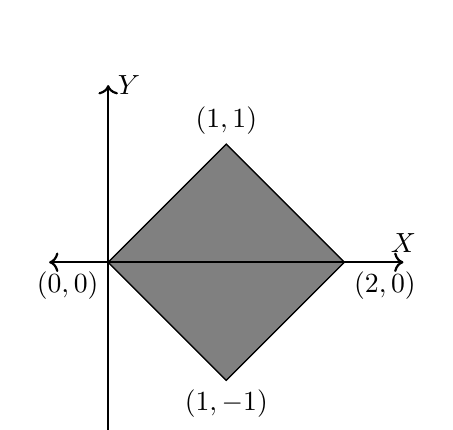
\begin{tikzpicture}[scale=1.5]
            \draw[fill=gray] (0, 0) -- (1, 1) -- (2, 0) -- (1, -1) -- (0,0);
            \draw [thick, <->] (-0.5, 0) -- (2.5, 0){};
            \draw [thick, <->] (0, -1.5) -- (0, 1.5);
            \draw (0, 0) -- (1, 1) -- (2, 0) -- (1, -1) -- (0,0);
            \node[above] at (2.5, 0) {$X$};
            \node[right] at (0, 1.5) {$Y$};
            \node[below left] at (0, 0) {$(0, 0)$};
            \node[below right] at (2, 0) {$(2, 0)$};
            \node[above] at (1, 1) {$(1, 1)$};
            \node[below] at (1, -1) {$(1, -1)$};
          \end{tikzpicture}
        \end{equation*}

      \item The joint density is given by the absolute value of the Jacobian determinant
        \begin{equation*}
          \det\!\left( \pder{(\omega_{1}, \omega_{2})}{(x, y)} \right)
        \end{equation*}
        with
        \begin{equation*}
          \omega_{1}(x, y) = {\left( \frac{x+y}{2} \right)}^{2}\quad\text{and}\quad \omega_{2}(x, y) = \frac{x-y}{2}.
        \end{equation*}
        We find
        \begin{equation*}
          \begin{vmatrix}
            \pder{\omega_{1}}{x} & \pder{\omega_{1}}{y} \\
            \pder{\omega_{2}}{x} & \pder{\omega_{2}}{y}
          \end{vmatrix}
          =
          \begin{vmatrix}
            \frac{x+y}{2} & \frac{x+y}{2} \\
            \frac{x}{2} & -\frac{y}{2}
          \end{vmatrix}
          = -\frac{1}{4} {(x+y)}^{2},
        \end{equation*}
        so
        \begin{equation*}
          f_{(X, Y)}(x, y) =
          \begin{cases}
            \frac{1}{4}{(x+y)}^{2}, &(x, y) \in (X, Y)(\Omega) \\
            0, &\text{otherwise}.
          \end{cases}
        \end{equation*}

        Since the function $f_{(X, Y)}$ is zero outside the range of $(X, Y)$, we have to choose the bounds of our integrals to accommodate this. We have
        \begin{equation*}
          P_{(X, Y)}(B) = \int_{0}^{1} dx \int_{-x}^{0} dy\ \frac{{(x + y)}^{2}}{4} = \frac{1}{48}.
        \end{equation*}
    \end{enumerate}
  \end{quote}
\end{example}

\begin{theorem}
  The random variables $X$ and $Y$ are independent if and only if
  \begin{equation*}
    P_{(X, Y)} = P_{X} \times P_{Y}.
  \end{equation*}
\end{theorem}

\subsection{Riesz representation theorem}
\begin{definition}[space of continuous bounded functions]
  \label{def:spaceofboundedlinearfunctions}
  For any topological space $(X, \tau)$, $C(X)$ denotes the \defn{space of bounded continuous functions} $X \to \R$. This is a real vector space.
\end{definition}

\begin{theorem}[Riesz representation theorem]
  \label{thm:rieszrepresentationtheorem}
  Let $[a, b] \subset \R$, and let $\Lambda\colon C([a, b]) \to R$ be a non-negative linear functional such that
  \begin{equation*}
    \Lambda(1) = 1.
  \end{equation*}

  Then there is a unique probability measure $\mu$ on the Borel $\sigma$-algebra $\mathcal{B}_{[a, b]}$ such that
  \begin{equation*}
    \Lambda(f) = \int_{[a, b]} f\ d\mu\qquad\text{for all }f \in C([a, b]).
  \end{equation*}
\end{theorem}

\begin{example}
  Consider the linear functional
  \begin{equation*}
    \Lambda\colon C([0, 1]) \to \R;\qquad f \mapsto \frac{1}{2}\left( \int_{[0, 1]} f\ dm + \sum_{n=1}^{\infty} {\left( \frac{1}{2} \right)}^{n} f\left( {\left( \frac{1}{3} \right)}^{n} \right) \right).
  \end{equation*}

  The functional $\Lambda$ is normalized since
  \begin{equation*}
    \Lambda(1) = \frac{1}{2}\left( \int_{[0, 1]} 1\ dm + \sum_{n=1}^{\infty} {\left( \frac{1}{2} \right)}^{n} \right) = \frac{1}{2}\left( 1 + 1 \right) = 1.
  \end{equation*}

  It is equivalent to integration with respect to the measure
  \begin{equation*}
    \frac{1}{2}\left( m + \sum_{n=1}^{\infty} \frac{1}{2^{n}} \delta_{{\left( \frac{1}{3} \right)}^{n}} \right).
  \end{equation*}
\end{example}

\section{The Radon-Nikodym theorem}
\begin{definition}[absolutely continuous]
  \label{def:absolutelycontinuous}
  Let $(\Omega, \mathcal{F})$ be a measurable space, and let $\mu$ and $\nu$ be measures on $(\Omega, \mathcal{F})$. We say that $\nu$ is \defn{absolutely continuous} with respect to $\mu$, and write $\nu \ll \mu$, if
  \begin{equation*}
    \mu(A) = 0 \implies \nu(A) = 0
  \end{equation*}
  for all $A \in \mathcal{F}$.
\end{definition}

\begin{note}
  Here is a way of remembering which way things go: the $\ll$ sorts of looks like the head of an double arrow, and it points the same way as the implication arrow. That is,
  \begin{equation*}
    \nu(A) = 0 \Longleftarrow \mu(A) = 0 \text{ for all }A \in \mathcal{F};\qquad \nu \ll \mu.
  \end{equation*}

  You know the thing is pointing the right way if it looks like a `less than'. No idea why.
\end{note}

\begin{example}
  Let $\nu$ be the measure defined on $([0, 1], \mathcal{M})$ by
  \begin{equation*}
    \nu(A) = \int_{A} x^{2}\ dm.
  \end{equation*}

  Then $\nu \ll m$, since
  \begin{equation*}
    m(A) = 0 \implies \int_{A} x^{2}\ dm = 0,
  \end{equation*}
  and $m \ll \nu$ since
  \begin{equation*}
    \int_{A} x^{2}\ dm = 0 \implies m(A) = 0.
  \end{equation*}
\end{example}

\begin{example}
  Let $\mu$ be the measure on $([0, 1], \mathcal{M}_{[0, 1]})$ defined by
  \begin{equation*}
    \mu = m + \delta_{\frac{1}{2}}.
  \end{equation*}

  Then if $\mu(A) = 0$, $m(A) = 0$ and $\delta_{\frac{1}{2}}(A) = 0$, so $m \ll \mu$.

  However, $m\left( \left\{ \frac{1}{2} \right\} \right) = 0$ but $\mu\left( \left\{ \frac{1}{2} \right\} \right) = 1$, so $\mu \not\ll m$.
\end{example}

\begin{theorem}[Radon-Nikodym]
  \label{thm:radonnikodym}
  Let $(\Omega, \mathcal{F})$ be a measurable space, and let $\mu$ and $\nu$ be measures on $(\Omega, \mathcal{F})$. Then $\nu \ll \mu$ if and only if there exists a non-negative measurable function $h\colon \Omega \to \R$ such that
  \begin{equation*}
    \nu(A) = \int_{A} h\ d\mu
  \end{equation*}
  for all $A \in \mathcal{F}$. We write
  \begin{equation*}
    h = \tder{\nu}{\mu},
  \end{equation*}
  and call $h$ the \defn{Radon-Nikodym derivative} of $\nu$ with respect to $\mu$.
\end{theorem}

\begin{example}
  Consider the measure space $(\R, \mathcal{M}, m)$, and consider a probability measure $P$ on $\R$. One can describe $P$ by its probability distribution function
  \begin{equation*}
    F(x) = P(X \leq x).
  \end{equation*}
\end{example}

\begin{corollary}
  \label{thm:changeofmeasures}
  Let $(\Omega, \mathcal{F})$ be a measurable space, and $\nu \ll \mu$ two measures. Then, for any measurable function $g\colon \Omega \to \R$ and any $A \in \mathcal{F}$,
  \begin{equation*}
    \int_{A} g\ d\nu = \int_{A} gh\ d\mu,
  \end{equation*}
  where $h = \tder{\nu}{\mu}$ is the Radon-Nikodym derivative, see \hyperref[thm:radonnikodym]{Theorem~\ref*{thm:radonnikodym}}.
\end{corollary}
\begin{proof}
  If we can prove the theorem in the case that $g$ is non-negative, then we can extend to the real case by splitting $g$ into positive and negative parts via positive decomposition (see, for example, \hyperref[def:integrablefunctionlebesgueintegral]{Definition~\ref*{def:integrablefunctionlebesgueintegral}} for an example of this). This is what we will do.

  We can always find a sequece of non-negative simple functions (\hyperref[def:simplefunction]{Definition~\ref*{def:simplefunction}}) $\varphi_{n}$ which increase monotonically to $g$ pointwise, i.e.\
  \begin{equation*}
    \varphi_{n} \uparrow g.
  \end{equation*}
  Therefore, by the monotone convergence theorem (\hyperref[thm:monotoneconvergencetheorem]{Theorem~\ref*{thm:monotoneconvergencetheorem}}),
  \begin{equation*}
    \lim_{n \to \infty} \int_{E} \varphi_{n}\ d\nu = \int \lim_{n \to \infty} \varphi_{n}\ d\nu = \int_{E} g\ d\nu.
  \end{equation*}
  This means that we have reduced the proof to one involving simple functions, which are much better behaved.

  Since simple functions only take on finitely many values, we can always write
  \begin{equation*}
    \varphi_{n} = \sum_{i} a_{i, n} \mathbb{I}_{E_{i, n}},
  \end{equation*}
  where $a_{i, n}$ is the $i$th value that $\varphi_{n}$ takes, and $E_{i, n}$ is the set on which $\varphi_{i, n}$ takes the value $a_{i, n}$. Then integration is simple: we have
  \begin{align*}
    \int_{A} \varphi_{n}\ d\nu &= \int_{A} \left( \sum_{i} a_{i, n} \mathbb{I}_{E_{i, n}} \right)\ d\nu \\
    &= \sum_{i} \int_{E} a_{i, n} \mathbb{I}_{E_{i, n}}\ d\nu \\
    &= \sum_{i} a_{i, n} \nu(E_{i, n} \cap E) \\
    &= \sum_{i} a_{i, n} \int_{E_{i, n} \cap E} d \nu \\
    &= \sum_{i} a_{i, n} \int_{E_{i, n} \cap E} h\ d\mu \\
    &= \sum_{i} \int_{E} h\,\mathbb{I}_{E_{i, n}} a_{i, n} \ d\mu \\
    &= \int_{E} h\,\varphi_{n}\ d\mu.
  \end{align*}
  Now, since $\varphi_{n} \uparrow g$ and $g$ and $h$ are both non-negative measurable functions, we must have that $\varphi_{n} h \uparrow gh$, hence by the monotone convergence theorem, we have
  \begin{equation*}
    \lim_{n \to \infty} \int_{E} \varphi_{n} h\ d\mu = \int_{E} \lim_{n \to \infty} \varphi_{n} h\ d\mu = \int_{E} gh\ d\mu.
  \end{equation*}
\end{proof}

\section{Conditional expectation}
For any random variable $X$, the sigma algebra generated by $X$, denoted $\mathcal{F}_{X}$ (see \hyperref[def:sigmaalgebrageneratedbyarandomvariable]{Definition~\ref*{def:sigmaalgebrageneratedbyarandomvariable}}) encodes a lot of information about $X$. For example, suppose one is to make a measurement of a physical quantity, and models the outcome by the random variable $X$. The accuracy of the measurement device controls the size of $\mathcal{F}_{X}$. If $X$ can only take on 2 values (for example, a particle being either on the left or the right of a container) then the $\sigma$-algebra $\mathcal{F}_{X}$ contains only four elements, and takes on the schematic form $\left\{ \emptyset, \text{left}, \text{right}, \Omega \right\}$. Increasing the resolution of the experiment (by, for example, further subdividing the box), increases the size of the $\sigma$-algebra; this reflects the fact that the measurement gave us more information.

Sometimes, the value that some random variable takes gives us information about the values that another random variable is likely to take. For example, if we make a measurement of the location of a particle at time $t$ and learn that it is on the left side of the box, and wait a short enough amount of time $\varepsilon$, the particle is more likely to still be on the left side of the box at time $t + \varepsilon$. This increase in information is formalized by the conditional expectation.

In principle, we can compute the contitional expectation no matter what the outcome of our previous experiment was. For example, given that the particle was in $X = 0$, $1$ side of the box a second ago, the expected value of the result of the future measurement of which side the particle is on can be expressed as a function of $0$, $1$. Thus, we can view the expected value of the future measurement (now a number between 0 and 1) as a function of the possible outcomes of the previous measurement. The conditional probability can also accomodate a situation in which we don't know which value the measurement took, but only that it took one of several values.

This sort of behavior: `any outcome or any combination thereof' is exactly what the $\sigma$-algebra $\mathcal{F}_{X}$ does! Therefore, the expected value of a random variable $X$ given some other random variable $Y$, denoted
\begin{equation*}
  \mathbb{E}(X | \mathcal{F}_{Y}),
\end{equation*}
should be given by a function $\Omega \to \R$ which is measurable with respect to $\mathcal{F}_{Y}$. The measurability with respect to $\mathcal{F}_{X}$ is exactly the condition that says that the conditional expectation is a function only of the outcome of the previous experiment, and does not contain any additional information.

What does a conditional expectation really tell us? If a previous measurement narrows down the state of our system to a subset $G$ of its state space, the conditional expectation value is the expected value of $X$ given that the system is somewhere in $G$. Mathematically, this means that for any element of the set of all possible amounts of information that $X$ can give us, i.e.\ for any $G \in \mathcal{F}_{X}$, we should have
\begin{equation*}
  \int_{G} \mathbb{E}(X | \mathcal{F}_{Y})\ dP = \int_{G} X\ dP.
\end{equation*}
This is all formalized in the following definition.

\begin{definition}[conditional expectation]
  \label{def:conditionalexpectation}
  Let $(\Omega, \mathcal{F}, P)$ be a probability space, and let $X$ be a random variable on $\Omega$. Let $\mathcal{G} \subset \mathcal{F}$ be a sub-$\sigma$-algebra. The \defn{conditional expectation} of $X$ relative to $\mathcal{G}$, denoted $\mathbb{E}(X | \mathcal{G})$, is a random variable on $\Omega$ defined by the following characteristics.
  \begin{enumerate}
    \item $\mathbb{E}(X | \mathcal{G})$ is $\mathcal{G}$-measurable, and

    \item $\int_{G} \mathbb{E}(X | \mathcal{G})\ dP = \int_{G} X\ dP$ for all $G \in \mathcal{G}$.
  \end{enumerate}
\end{definition}

\begin{note}
  If the $\sigma$-algebra with respect to which we are taking the conditional expectation is derived from a random variable $X$, we will often write $\mathbb{E}(Y|X)$ instead of $\mathbb{E}(Y|\mathcal{F}_{X})$.
\end{note}

\begin{example}
  The result of a roll of a fair die is modelled by a random variable $X$. Let
  \begin{equation*}
    Z =
    \begin{cases}
      0, & X\text{ even}\\
      1, & X\text{ odd}.
    \end{cases}
  \end{equation*}

  Here, we are working with the probability space $(\Omega, \mathcal{F}, P)$, where
  \begin{equation*}
    \Omega = \{ 1, 2, 3, 4, 5, 6 \};\qquad\mathcal{F}\text{ is the discrete $\sigma$-algebra on $\Omega$};\qquad P(A) = \frac{\abs{A}}{6}.
  \end{equation*}

  The $\sigma$-algebra $\mathcal{F}_{Z}$ is
  \begin{equation*}
    \mathcal{F}_{Z} = \left\{ \emptyset, \{ 1,3,5\}, \{2,4,6\}, \Omega \right\}.
  \end{equation*}

  Let us calculate $\mathbb{E}(X | Z)$. The conditions of \hyperref[def:conditionalexpectation]{Definition~\ref*{def:conditionalexpectation}} tell us the following:
  \begin{enumerate}
    \item Since $\mathbb{E}(X | Z)$ must be measurable with respect to $\mathcal{F}_{Z}$, it must take the form
      \begin{equation*}
        \mathbb{E}(X | Z)(\omega) =
        \begin{cases}
          a, & \omega \in \{ 1, 3, 5 \} \\
          b, & \omega \in \{ 2, 4, 6 \}.
        \end{cases}
      \end{equation*}

    \item We must have
      \begin{equation*}
        \int_{\{1, 3, 5\}} \mathbb{E}(X | Z)\ dP = \int_{\{1, 3, 5\}} X\ dP
      \end{equation*}
      and
      \begin{equation*}
        \int_{\{2, 4, 6\}} \mathbb{E}(X | Z)\ dP = \int_{\{2, 4, 6\}} X\ dP
      \end{equation*}

      These integrals are really sums in disguise (see \hyperref[eg:lebesgueintegralcanbesumagain]{Example~\ref*{eg:lebesgueintegralcanbesumagain}}); we have
      \begin{align*}
        \int_{\{1, 3, 5\}} \mathbb{E}(X | Z)\ dP &= \int_{\{1, 3, 5\}} X\ dP \\
        \frac{1}{6} \sum_{\omega \in \{1, 3, 5\}} \mathbb{E}(X | Z)(\omega) &= \frac{1}{6} \sum_{\omega \in \{1, 3, 5\}} X(\omega) \\
        \frac{1}{2} \cdot a &= \frac{3}{2}, \\
      \end{align*}
      so $a = 3$. An almost identical calculation tells us that $b = 4$. Thus,
      \begin{equation*}
        \mathbb{E}(X | Z) =
        \begin{cases}
          3, & \omega \in \{ 1, 3, 5 \} \\
          4, & \omega \in \{ 2, 4, 6 \}.
        \end{cases}
      \end{equation*}
  \end{enumerate}
\end{example}

\begin{theorem}
  The conditional expectation always exists and is unique up to agreement almost everywhere. That is, for $(\Omega, \mathcal{F}, P)$ a probability space, $X$ a random variable on $\Omega$ and $\mathcal{G}$ a subalgebra of $\mathcal{F}$, the conditional expectation $\mathbb{E}(X | G)$ is uniquely defined almost everywhere.
\end{theorem}
\begin{proof}
  First, we show existence. Perform positive decomposition on $X$, so
  \begin{equation*}
    X = X^{+} - X^{-}.
  \end{equation*}

  Define measures $\nu^{+}$ and $\nu^{-}$ on $(\Omega, \mathcal{G})$ as follows:
  \begin{equation*}
    \nu^{\pm}(G) = \int_{G} X^{\pm}\ dP
  \end{equation*}
  for any $G \in \mathcal{G}$. Also define $\mu$ to be the restriction of $P$ to $\mathcal{G}$.

  If $G_{0} \in \mathcal{G}$ is null with respect to $P$, then
  \begin{equation*}
    \nu^{\pm}(G_{0}) = \int_{G_{0}} X^{\pm}\ d\mu = \int_{G_{0}} X^{\pm}\ dP = 0,
  \end{equation*}
  so $\nu^{\pm} \ll \mu$. Thus, the Radon-Nikodym theorem (\hyperref[thm:radonnikodym]{Theorem~\ref*{thm:radonnikodym}}) tells us that there exist non-negative measurable functions $h^{\pm}$ such that
  \begin{equation*}
    \nu^{\pm}(B) = \int_{B} h^{\pm}\ d\mu\quad\text{for all }B \in\mathcal{B}.
  \end{equation*}

  Now,
  \begin{align*}
    \nu^{+}(G) - \nu^{-}(G) &= \int_{G} X^{+}\ d\mu - \int_{G} X^{-}\ d\mu \\
    &= \int_{G} X\ d\mu\\
    &= \int_{G} X\ dP,
  \end{align*}
  but
  \begin{equation*}
    \nu^{+}(G) - \nu^{-1}(G) = \int_{G} \left( h^{+} - h^{-} \right) dP,
  \end{equation*}
  so for any $G \in \mathcal{G}$,
  \begin{equation*}
    \int_{B} X\ dP = \int_{B} h^{+} - h^{-}\ dP.
  \end{equation*}
\end{proof}

\begin{lemma}[properties of the conditional expectation]
  \label{lemma:propertiesoftheconditionalexpectation}
  $\,$
  \begin{enumerate}
    \item $\E(\E(X | \mathcal{G})) = \E(X)$.

    \item If $X$ is $\mathcal{G}$-measurable, then $\E(X | \mathcal{G}) = X$.

    \item If $X$ is independent of $\mathcal{G}$, then $\E(X|\mathcal{G}) = \E(X)$

    \item $\E(aX+bY|\mathcal{G}) = a\E(X|\mathcal{G}) + b\E(Y|\mathcal{G})$.

    \item If $X_{n}$, $n = 1, 2, \ldots$ are non-negative random variables increasing to $X$ almost everywhere, then $\E(X_{n}|\mathcal{G}) = \E(X|\mathcal{G})$ almost everywhere.

    \item If $Y$ is $\mathcal{G}$-measurable and $XY$ is integrable, then $\mathbb{E}(XY|\mathcal{G}) = Y\cdot\mathbb{E}(X|G)$.

    \item If $\mathcal{H} \subset \mathcal{G}$, then $\mathbb{E}(\mathbb{E}(X | \mathcal{G}) | \mathcal{H}) = \mathbb{E}(X | \mathcal{H})$.
  \end{enumerate}
\end{lemma}
%\begin{proof}
%  $\,$
%  \begin{enumerate}
%    \item By definition, we have that for any $A \in \mathcal{G}$,
%      \begin{equation*}
%        \int_{A} \E(X | \mathcal{G})\ dP = \int_{A} X\ dP.
%      \end{equation*}
%      Since $\Omega \in \mathcal{G}$ by definition, we are guaranteed that
%      \begin{equation*}
%        \int_{\Omega} \E(X | \mathcal{G})\ dP = \int_{\Omega} X\ dP = \E(X).
%      \end{equation*}

%    \item We have the identity
%      \begin{equation*}
%        \int_{G} \E(X | \mathcal{G})\ dP = \int_{G} X\ dP
%      \end{equation*}
%      for any $G \in \mathcal{G}$.

%    \item

%    \item By definition, the conditional expectation $\E(aX+bY|\mathcal{G})$ must be $\mathcal{G}$-measurable and satisfy
%      \begin{equation*}
%        \int_{G} \E(aX + bY|\mathcal{G})\ dP = \int_{G} aX + bY\ dP\qquad\text{for any }G \in \mathcal{G}.
%      \end{equation*}

%      The function $a\E(X | \mathcal{G}) + b\E(Y | \mathcal{G})$ is $\mathcal{G}$-measurable, and
%      \begin{align*}
%        \int_{G} a\E(X|\mathcal{G}) + b\E(Y | \mathcal{G})\ dP &= a\int_{G} \E(X|\mathcal{G})\ dP + b\int_{G}\E(Y|\mathcal{G})\ dP \\
%        &= a\int_{G} X\ dP + b\int_{G} Y\ dP \\
%        &= \int_{G} aX + bY\ dP,
%      \end{align*}
%      so $a\E(X | \mathcal{G}) + b\E(Y | \mathcal{G})$ is a conditional expectation of $aX+bY$ relative to $\mathcal{G}$.

%    \item By the monotone convergence theorem (\hyperref[thm:monotoneconvergencetheorem]{Theorem \ref*{thm:monotoneconvergencetheorem}}),
%  \end{enumerate}
%\end{proof}

\begin{example}
  On the probability space $\left( [-1, 1], \mathcal{B}_{[-1, 1]}, \frac{1}{2}m \right)$, consider the random variable $X(\omega) = \omega^{2}$. The $\sigma$-algebra generated by $X$ is given by
  \begin{equation*}
    \left\{ A \cup (-A)\,\big|\, A \in \mathcal{B}_{[-0, 1]} \right\}.
  \end{equation*}

  For any random variable $Y$ on $[-1, 1]$, the conditional expectation $\mathbb{E}(Y|X)$ is given by
  \begin{equation*}
    \mathbb{E}(Y|X)(\omega) = \frac{Y(\omega) - Y(-\omega)}{2}.
  \end{equation*}
\end{example}

\section{Random processes}
\begin{notation}
  Let $\mathcal{F}_{i}$, $i = 1$, $2$, \dots, $n$, be $\sigma$-algebras on a set $\Omega$. Denote by
  \begin{equation*}
    \bigwedge_{i} \mathcal{F}_{i} = \mathcal{F}_{1} \wedge \mathcal{F}_{2} \wedge \cdots \wedge \mathcal{F}_{n}
  \end{equation*}
  the $\sigma$-algebra generated by the set $\bigcup_{i} \mathcal{F}_{i}$, i.e.\ the smallest $\sigma$-algebra which contains all the $\mathcal{F}_{i}$.
\end{notation}

\begin{definition}[discrete-time random process]
  \label{def:discretetimerandomprocess}
  A \defn{discrete-time random process} (or \emph{DTRP}) with real values on a probability space $(\Omega, \mathcal{F}, P)$ is a function
  \begin{equation*}
    X_{t}(\omega): \{1, 2, \ldots, n\} \times \Omega \to \R
  \end{equation*}
  such that for each $t_{0} \in \{1, 2, \ldots, n\}$, $\mathcal{F}_{t_{0}}(\omega)$ is a random variable on $(\Omega, \mathcal{F}, P)$. For a fixed $\omega \in \Omega$, the sequence
  \begin{equation*}
    \left\{ X_{1}(\omega), X_{2}(\omega), \ldots, X_{n}(\omega) \right\}
  \end{equation*}
  is called the \defn{sample path} (or \emph{trajectory}) or $\omega$.
\end{definition}

\begin{definition}[filtration, adapted process, natural]
  \label{def:filtration}
  A collection $\{\mathcal{F}_{t}\}$ of $\sigma$-algebras on a probability space $(\Omega, \mathcal{F}, P)$ is called a \defn{filtration} if $\mathcal{F}_{t} \subset \mathcal{F}_{t + 1} \subset \mathcal{F}$ for all $t \in \{1, 2, \ldots, n\}$. A process $X$ is \defn{adapted} to a filtration $\{\mathcal{F}_{t}\}$ if $X_{t}$ is $\mathcal{F}_{t}$-measurable for all $t$. The quadruple $(\Omega, \mathcal{F}, \{\mathcal{F}_{i}\}, P)$ is called a \defn{filtered} probability space. The \defn{natural} filtration is defined by
  \begin{equation*}
    \mathcal{F}_{t} = \bigwedge_{i=1}^{t}\mathcal{F}_{X_{i}}.
  \end{equation*}
\end{definition}

\begin{definition}[filtered probability space]
  \label{def:filteredprobabilityspace}
  A \defn{filtered probability space} is a quadruple
  \begin{equation*}
    (\Omega, \mathcal{F}, \{ \mathcal{F}_{t}, P \}),
  \end{equation*}
  where $(\Omega, \mathcal{F}, P \})$ is a probability space and $\{ \mathcal{F}_{t} \}$ is a filtration.
\end{definition}

\begin{lemma}
  Here is a collection of results that will be useful.
  \begin{enumerate}
    \item Let $(\Omega, \mathcal{F}, \{ \mathcal{F}_{t} \}, P)$ be a filtered probability space, and let $X$ be a DTRP which is adapted to $\{ \mathcal{F}_{i} \}$. Then $X_{t}$ is $\mathcal{F}_{s}$ measurable for all $s \geq t$.
  \end{enumerate}
\end{lemma}
\begin{proof}
  $\,$
  \begin{enumerate}
    \item Since $\mathcal{F}_{t} \subset \mathcal{F}_{s}$ for all $s \geq t$, by \hyperref[lemma:functionalsomeasurablewithrespecttobiggersigmaalgebra]{Lemma~\ref*{lemma:functionalsomeasurablewithrespecttobiggersigmaalgebra}}, $X_{t}$ is $\mathcal{F}_{s}$ measurable for all $s \geq t$.
  \end{enumerate}
\end{proof}

\begin{definition}[martingale, submartingale, supermartingale]
  \label{def:subsupermartingale}
  A real-valued process $X$ with $\mathbb{E}(|X_{t}|) < \infty$ for all $t$ and adapted to a filtration $\{\mathcal{F}_{t}\}$ is called an \defn{$\mathcal{F}_{t}$-martingale} if $\mathbb{E}(X_{t+s}|\mathcal{F}_{t}) \overset{\mathrm{a.e.}}{=} X_{t}$ for all $s$, $t$. It is called a \defn{submartingale} if $\mathbb{E}(X_{t+s}|\mathcal{F}_{t}) \overset{\mathrm{a.e.}}{\geq} X_{t}$, and a \defn{supermartingale} if $\mathbb{E}(X_{t+s}|\mathcal{F}_{t}) \overset{\mathrm{a.e.}}{\leq} X_{t}$.
\end{definition}

\begin{note}
  For me, this terminology is confusing. Na\"{\i}vely, a \emph{submartingale} would be a process for which the average value decreased over time, and a \emph{supermartingale} a process for which the average value increased; this is not the case. Oh well.
\end{note}

\begin{corollary}
  Let $X$ be an an adapted, real-valued process on a filtered probability space $(\Omega, \mathcal{F}, \{ \mathcal{F}_{t} \}, P)$ with $\E(\abs{X_{t}}) < \infty$ for all $t \in \{ 1, 2, \ldots \}$. Suppose that for all $t \in \{ 1, 2, \ldots \}$, $\E(X_{t+1}|\mathcal{F}_{t}) \overset{\mathrm{a.e.}}{=} X_{t}$. Then $X$ is martingale.
\end{corollary}
\begin{proof}
  Follows trivially by induction. More concretely,
  \begin{equation*}
    X_{t} = \E(X_{t+1}|\mathcal{F}_{t}) = \E(\E(X_{t + 2}|\mathcal{F}_{t + 1})|\mathcal{F}_{t}) = \cdots = \E(\E(\cdots \E(X_{t + s}|\mathcal{F}_{t+s-1})|\mathcal{F}_{t+s-2})\cdots |\mathcal{F}_{t}).
  \end{equation*}

  Property 7 of \hyperref[lemma:propertiesoftheconditionalexpectation]{Lemma~\ref*{lemma:propertiesoftheconditionalexpectation}} tells us that if $\mathcal{H} \subset \mathcal{G}$, then $\mathbb{E}(\mathbb{E}(X | \mathcal{G}) | \mathcal{H}) = \mathbb{E}(X | \mathcal{H})$. Since $\{ \mathcal{F}_{t} \}$ is a filtration, $\mathcal{F}_{t + s} \in \mathcal{F}_{t}$ for all $t$ and $s$. Thus, the above expression collapses to
  \begin{equation*}
    \E(X_{t+s}|\mathcal{F}_{t}),
  \end{equation*}
  so $\E(X_{t+s}|\mathcal{F}_{t}) = X_{t}$, and $X_{t}$ is martingale.
\end{proof}

\begin{example}
  Consider a gambler betting on the flip of a coin. If the coin comes up heads, the gambler wins $\$ 1$. If the coin comes up tails, the gambler loses $\$1$. Consider the wealth $W$ of the gambler after the $t^\mathrm{th}$ toss. This is a DTRP\@.

  \begin{itemize}
    \item If the coin is fair, $W$ is a martingale.

    \item If the coin lands on heads more often than tails, so the gambler wins on average, then $W$ is a submartingale.

    \item If the coin lands on tails more often than heads, $W$ is a supermartingale.
  \end{itemize}
\end{example}

\begin{example}
  Imagine a 1-dimensional box $[0, 1]$ filled with a gas. At any time
  \begin{equation*}
    t \in \{ 0, 1, \ldots, n \},
  \end{equation*}
  the position of a particular gas particle can be modelled by a random variable $X_{t}$. This is a DTRP with filtration
  \begin{equation*}
    \mathcal{F}_{t} = \mathcal{M}_{[0, 1]}\qquad\text{for all } t.
  \end{equation*}
\end{example}

\begin{thebibliography}{50}
    \bibitem{measurablesetsarelimitpoints} Jun Tanaka and Peter F. McLoughlin.
    \textit{A Realization of Measurable Sets as Limit Points}.
    arXiv:0712.2270 [math.FA]
\end{thebibliography}

\end{document}
